\documentclass{article}
\usepackage{commands} % Required for inserting images

\title{Math 13 Lecture Notes}
\author{Timothy Cho}
\date{December 2023}

\begin{document}

\begin{titlepage}
    \begin{center}
        \vspace*{1cm}
            
        \Huge
        \textbf{UC Irvine Math 13 Winter 2022}
        
        \vspace{0.1 cm}
        \huge
        \textbf{Introduction to Abstract Mathematics}
        \vspace{0.4cm}
            
        \vspace{1.5cm}
        \Large    
        \text{Professor: Erik Walsberg}

        \text{Teaching Assistant: Cheuk-Wai Yau}
        
        \text{Notes: Timothy Cho}
            
        \vfill
            

            
        \vspace{0.8cm}
            

        \Large
        January 2024

        Lecture Note Series \#\textbf{4}
            
    \end{center}
\end{titlepage}
\section*{Introduction}
These notes are roughly sorted chronologically, but sections are mainly organized by topic. The scope of these notes cover most lectures and some discussion. We should note that this iteration of Math 13 was quite unorthodox; hence, these do not exactly line up with the UC Irvine Math 13 official course notes (by Neil Donaldson); however, the material here is worth their weight in paper, at least for a review of Math 13. Some interesting exercises are included at the back of these notes to aid practice and readability.

\section{Propositional Logic}
In this section, we introduce the notion of a \textit{proposition}, and we learn the basic logical connectives that will occur in this course.
\begin{definition}
A \textit{proposition} is a statement that is definitively either true or false.
\end{definition}
For example, ``the sum of $2$ and $2$ is $4$" is a true proposition, whereas ``Eggs are tasty" is not even a proposition, as it is an \textit{opinion} that is not definitively true or false. We represent propositions using capital letters, usually $P$ or $Q$, the trueness or the falsity of a proposition is called its \textit{truth value}. We write $|P| = 1$ to mean that $P$ is true, and $|P| = 0$ to mean that $P$ is false. We also write $P\equiv Q$ whenever $P$ and $Q$ have the same truth value. Doing so, we can build longer propositions out of short ones, using logical connectives.
\begin{definition}
Let $P$ and $Q$ be propositions. We define these propositions in terms of the truth values for $P$ and $Q$:
\begin{enumerate}
    \item The \textit{conjunction} $P\land Q$, read ``$P$ and $Q$", is true exactly when $P$ and $Q$ are both true. It is false otherwise.
    \item Then \textit{disjunction} $P\lor Q$, read ``$P$ or $Q$", is false exactly when $P$ and $Q$ are both false. It is true otherwise.
    \item The \textit{negation} $\lnot P$, read ``not $P$," is true when $P$ is false, and false when $P$ is true.
    \item The \textit{implication} $P\implies Q$, read ``if $P$ then $Q$," is false exactly when $P$ is true and $Q$ is false. It is true otherwise.
    \item The \textit{equivalence} $P\iff Q$, read ``$P$ if and only if $Q$," is true whenever $P\equiv Q$. It is false otherwise.
\end{enumerate}
\end{definition}
We note that the equivalence is sometimes called the \textit{biconditional}. We leave it to the reader to verify these fundamental identities.
\begin{theorem}[Properties of Logical Connectives]
Let $P, Q,$ and $R$ be propositions. Then the following properties hold:
\begin{enumerate}
    \item[$1.$] Associativity of Conjunction: $(P\land Q)\land R \equiv P \land (Q\land R)$.
    \item[$2.$] Associativity of Disjunction: $(P\lor Q)\lor R\equiv P\lor (Q\lor R)$.
    \item[$3.$] Distributivity I: $P \land (Q\lor R) \equiv (P\land Q) \lor (P \land R)$.
    \item[$4.$] Distributivity II: $P\lor (Q\land R) \equiv (P\lor Q) \land (P\lor R)$.
    \item[$5.$] Double Negation Property: $\lnot(\lnot P) \equiv P$.
    \item[$6.$] Commutativity of Conjunction: $P\land Q \equiv Q\land P$.
    \item[$7.$] Commutativity of Disjunction: $P\lor Q \equiv Q\lor P$.
    \item[$8.$] Decomposition of Implication: $(P \implies Q) \equiv (\lnot P) \lor Q \equiv \lnot (P \land \lnot Q)$.
    \item[$9.$] DeMorgan I: $\lnot (P\lor Q) \equiv \lnot P \land \lnot Q$.
    \item[$10.$] DeMorgan II: $\lnot (P\land Q) \equiv \lnot P\lor \lnot Q$.
    \item[$11.$] Decomposition of Equivalence: $(P\iff Q) \equiv (P\implies Q)\land (Q\implies P)$.
    \item[$12.$] Contrapositive: $(P\implies Q) \equiv (\lnot Q\implies \lnot P)$.
\end{enumerate}
\end{theorem}
With all of this being said, one fine detail should not be missed. Recall that we write $P\equiv Q$ whenever $P$ and $Q$ share the same truth value; we vocalize this as saying ``$P$ is \textit{(logically) equivalent} to $Q$." \textbf{However, $P$ is not necessarily equal to $Q$}! For example, if $P$ is the statement $0=3$, and $Q$ is the statement ``the derivative of $x^2$ is $e^x$," then clearly $P\equiv Q$ as both statements are false, but $P\neq Q$ in that the statements $P$ and $Q$ are quite literally different words. In a slightly more subtle way, $P\land Q$ and $Q\land P$ are \textit{not} the same statement in that the \textit{order} of the words are different, but the notion of logical equivalence allows us to consider $P\land Q$ and $Q\land P$ to be ``basically equivalent" for lack of a better term. Notice that if indeed $P\equiv Q$, then $P$ and $Q$ are also ``basically equivalent" even if the sentential content in $P$ and $Q$ are vastly different: this is the limit to the logical system we are using, as it cannot distinguish propositions based on ``related-ness," but merely on truth alone.

Here are some exercises to work through.
\begin{exercise}
Let $P$ and $Q$ be propositions. We define the \textit{exclusive disjunction} $P + Q$, read ``$P$ exclusive or $Q$," to be true whenever exactly one of $P$ and $Q$ are true, and false otherwise. Prove the following for all propositions $P, Q, R$:
\begin{itemize}
    \item[(a)] $P+Q \equiv \lnot (P\iff Q)$.
    \item[(b)] $P+Q = Q+P$.
    \item[(c)] $(P+Q)+R \equiv P + (Q+R)$.
    \item[(d)] $P \land (Q+R) \equiv (P\land Q) + (P\land R)$.
\end{itemize}
\end{exercise}
\begin{exercise}
Let $P$ and $Q$ be propositions. We define the \textit{not conjunction} $P \uparrow Q$, read ``$P$ nand\footnote{That is, ``not and."} $Q$," to be true whenever $P\land Q$ is false, and false whenever $P\land Q$ is true. That is, we have
$$P\uparrow Q \equiv \lnot (P\land Q).$$
Prove the following for all propositions $P$ and $Q$:
\begin{itemize}
    \item[(a)] $\lnot P \equiv P\uparrow P$.
    \item[(b)] $P\land Q \equiv (P\uparrow Q) \uparrow (P \uparrow Q)$.
    \item[(c)] $P\lor Q \equiv (P\uparrow P) \uparrow (Q\uparrow Q)$.
\end{itemize}
This exercise shows that the $\uparrow$ operation is \textit{functionally complete}: all of our familiar operators can be written solely in terms of just the $\uparrow$.
\end{exercise}
\newpage

\section{Sets I: Basic Definitions}
In this class, logic is important as we need to discuss sets, which in some extent depend on whether a certain thing is ``inside" the set or not.\footnote{A more modern framework is that of \textit{category theory}, which is not as concerned about the stuff inside a set.} To do this, we will make the following definition of a set, which is good enough for our purposes.
\begin{definition}
A \textit{set} $S$ is any collection of objects, called \textit{elements} of the set. If $x$ is included inside $S$, then we write $x\in S$ (read ``$x$ is in $S$") to denote this relationship. Similarly, if $x$ is not included inside $S$, we write $x\not\in S$.
\end{definition}
What an object is really depends on the context. For example, $\{2, 5\}$ is a set containing the numbers $2$ and $5$, and so is the \textit{singleton set} $\{e^x\}$, containing a function. We note that sets can contain other sets, such as $\set{3, \pi, \set{f, j}}$. Sets do not contain duplicate elements, so $\set{3, 4, 3}$ is the same set as $\set{3, 4}$. There is also a unique set containing nothing:
\begin{definition}
The \textit{empty set}, denoted $\varnothing$, is the set containing no elements: $\varnothing := \set{}$.
\end{definition}

We are able to specify elements of a set by explicitly listing them out (as we did above), or by using \textit{set builder notation}:
$$A = \{x: P_x \textrm{ is true}\},$$
where $P_x$ is some proposition that depends on the $x$ you choose. For example, consider the set
$$E = \{x: x \textrm{ is an integer multiple of }3\} = \{..., -6, -3, 0, 3, 6,...\},$$
where $P_x$ is the proposition ``$x$ is a multiple of $3$." The set $E$ thus contains exactly the elements $x$ such that $P_x$ is true; i.e., it contains all multiples of $3$ and nothing else. Of course, now that we have propositions, we can build new sets out of old just like we built new propositions out of smaller ones.
\begin{definition}
Let $A$ and $B$ be sets. We define these new sets in terms of $A$ and $B$:
\begin{enumerate}
    \item The \textit{union} $A\cup B$ is the set $A\cup B := \set{x: (x\in A) \lor (x\in B)}.$
    \item The \textit{intersection} $A\cap B$ is the set $A\cap B := \set{x: (x\in A)\land (x\in B)}$.
    \item The \textit{set difference} $A\setminus B$ is the set $A\setminus B := \set{x: (x\in A)\land (x\not \in B)}$.
    \item The \textit{set sum} $A\oplus B$ is the set $A\oplus B := (A\cup B) \setminus (A\cap B)$.
\end{enumerate}
\end{definition}
We would also like to determine the ``size" of two sets. There are two obvious ways to do this: count the number of elements in the set, leading to a notion of \textit{cardinality} (which we will explore in detail later), or seeing if one set is entirely contained in another. Hence, we make the following definition.
\begin{definition}
Let $A, B$ be sets. We say that $A$ \textit{is a subset of} $B$ if $x\in A$ implies $x\in B$, for any $x\in A$. We write $A\subseteq B$ to denote this relationship. In the case that we want to stress $A\neq B$, we will write $A\subsetneq B$ and say that $A$ \textit{is a proper subset of} $B$.
\end{definition}
Now, we can also define what it means for two sets to be equal:
\begin{definition}
Let $A,B$ be sets. Then $A = B$ precisely if $A$ and $B$ contain the exact same elements.
\end{definition}
For example, if $A = \{x: x \text{ is an even prime}\}$ and $B = \{2\}$, then $A = B$. That is, $A$ and $B$ are just names that represent the same object: the singleton set $\{2\}$. We also get the following proposition.
\begin{proposition}
Let $A,B$ be sets. Then $A = B$ if and only if both $A\subseteq B$ and $B\subseteq A$ are satisfied.
\end{proposition}
Hence, in order to prove that two sets are equal, we show that they are mutually subsets of each other. From here, we get the following properties that should look a lot like what we did for logic.
\begin{proposition}[Properties of Set Constructions]
Let $A, B,$ and $C$ be sets. Then the following properties hold:
\begin{itemize}
    \item[$1.$] Associativity of Intersection: $(A\cap B) \cap C = A \cap (B\cap C)$.
    \item[$2.$] Associativity of Union: $(A\cup B) \cup C = A \cup (B\cup C)$.
    \item[$3.$] Distributivity I: $A \cap (B \cup C) = (A \cap B) \cup (A\cap C)$.
    \item[$4.$] Distributivity II: $A\cup (B \cap C) = (A \cup B)\cap (A\cup C)$.
    \item[$5.$] Commutativity of Intersection: $A\cap B = B\cap A$.
    \item[$6.$] Commutativity of Union: $A\cup B = B\cup A$.
\end{itemize}
\end{proposition}
We note that we are dealing with true, honest \textit{equality} here, not just \textit{equivalence} as with the logic case. Also, a lot of the time, we will be thinking of sets as residing in some ``collection of everything," usually denoted $\mathcal U$. We call $\mathcal U$ the \textit{universal set}, which contains all the sets that we are interested in.\footnote{The logician will have trouble accepting this, but this is good enough for our purposes.} If we accept the existence of such a universal set $\mathcal U$, we make the following definitions.
\begin{definition}
Let $A$ be a set contained in some universal set $\mathcal U$; i.e., $A\subseteq\mathcal U$. We define the \textit{complement} of $A$ to be the set $A^c := \mathcal U\setminus A$.
\end{definition}
That is, the complement of $A$ is the set of everything not in $A$, where our ``everything" depends on what our universal set is. From this, we get a few more propositions that look a lot like logic once more.
\begin{proposition}[Properties of the Complement]
Let $A, B$ be contained in some universal set $\mathcal U$. Then the following properties hold:
\begin{enumerate}
    \item[$1.$] Double Complement Property: $(A^c)^c = A$.
    \item[$2.$] DeMorgan I: $(A\cup B)^c = A^c \cap B^c$.
    \item[$3.$] DeMorgan II: $(A\cap B)^c = A^c \cup B^c$.
\end{enumerate}
\end{proposition}

Here are some exercises for the reader to think about.
\begin{exercise}
Let $A$ and $B$ be sets. Show that $A\cup B$ is the ``smallest" set containing both $A$ and $B$; i.e., if $S$ is a set with $A\subseteq S$ and $B\subseteq S$, then we have $A\cup B\subseteq S$.
\end{exercise}
\begin{exercise}
Let $A$ and $B$ be sets. Show that $A\cap B$ is the ``largest" set containing elements which are both in $A$ and $B$; i.e., if $S$ is a set such that $S\subseteq A$ and $S\subseteq B$, then $S\subseteq A\cap B$.
\end{exercise}
\begin{exercise}
Prove the following for sets $A, B,$ and $C$. [Hint: use the exclusive disjunction.]
\begin{itemize}
    \item[(a)] $A\oplus (B\oplus C) = (A\oplus B)\oplus C$;
    \item[(b)] $A\oplus B$ = $B\oplus A$;
    \item[(c)] $A\oplus\varnothing = A$;
    \item[(d)] $A\cap (B\oplus C) = (A\cap B)\oplus (A\cap C)$.
\end{itemize}
This exercise shows that $\oplus$ and $\cap$ are set analogues of $+$ and $\times$ over the real numbers.
\end{exercise}
\begin{exercise}
Prove that for all sets $A,B$, one has $A\oplus B = (A\setminus B)\cup (B\setminus A)$.
\end{exercise}

\section{Sets II: Advanced Constructions and Cardinality}
We have already seen the sum and difference of two sets $A$ and $B$. We will now define the notion of a \textit{product} of sets.
\begin{definition}
Let $A,B$ be sets. Then the \textit{Cartesian product} of $A$ and $B$, denoted $A\times B$, is the set of all \textit{ordered pairs} where the first coordinate comes from $A$ and the second coordinate comes from $B$:
$$A\times B := \set{(x,y): (x\in A)\land (y\in B)}.$$
\end{definition}
Notice that the elements of $A\times B$ fundamentally ``look different" than that of $A$ and $B$: those in $A$ and $B$ are specifically elements, while the elements in $A\times B$ are specifically ordered pairs of elements. Of course, we will also define Cartesian products of multiple sets in the obvious way: if $A_1, \ldots, A_n$ are sets, then we write
$$A_1\times A_2\times\cdots\times A_n := \set{(x_1, \ldots, x_n): (x_1\in A_1)\land \cdots\land (x_n\in A_n)}.$$
To see why $A\times B$ is called a ``product," we introduce the notion of cardinality.  
\begin{definition}\label{cardinality}
Let $A$ be a set. The \textit{cardinality} of $A$, denoted $|A|$, is the number of elements that $A$ contains. We say that $A$ is \textit{finite} if $|A|$ is finite, and $A$ is \textit{infinite} otherwise.
\end{definition}

Our next theorem tells us that Cartesian products cause the cardinality to be multiplicative.
\begin{theorem}
Let $A, B$ be both finite sets. Then $|A\times B| = |A| \cdot |B|$.
\end{theorem}
\begin{proof}
By definition, we have $A\times B = \set{(x,y): x\in A \land y\in B}$. That is, every element of $A\times B$ can be thought of as a choice of an element from $A$, followed by a choice of an element from $B$. If we have $|A| = m$ and $|B| = n$, we see that we have $m\cdot n$ choices for ordered pairs. This completes the proof.
\end{proof}

Our next construction gives us an analogue to \textit{exponentiation} for sets.
\begin{definition}
Let $A$ be a set. Then the \textit{power set} of $A$, denoted $\mathcal P(A)$, is the set of all subsets of $A$:
$$\mathcal P(A) := \set{X: X\subseteq A}.$$
\end{definition}
Notice that the power set is a \textit{set of sets}! The elements themselves are sets: for example, if $A = \{1, 2, 3\}$, then we see that $\{2,3\}\in X$. \textbf{It would be incorrect to write $\{2,3\}\subseteq X$}, as $X$ is a set of sets. We have the following theorem about the size of a power set.

\begin{theorem}\label{power set size}
Let $A$ be a finite set. Then $|\mathcal P(A)| = 2^{|A|}$.
\end{theorem}
It is for this reason why we can think of a power set as raising $2$ to some \textit{power}.
\begin{proof}
Let $|A| = n$, so we write $A = \{a_1, \ldots, a_n\}$. [We are of course assuming the $a_i$ are distinct.] We build a subset $B$ of $A$ by running through the $a_i$ and deciding whether each $a_i$ is in $B$ or not. This is a \textit{binary choice}: $a_i\in B$, or $a_i\not\in B$. Since we have $n$ choices to make, we end up with $2^n$ outcomes. Hence $|\mathcal P(A)| = 2^n = 2^{|A|}$.
\end{proof}
\begin{example}
If $A = \varnothing$, then $\varnothing \subseteq \varnothing$. Hence $P(\varnothing) = \{\varnothing\}$, which has cardinality $2^0 = 1$, as expected.
\end{example}
Here is perhaps a simpler way to think about the proof of Theorem \ref{power set size}. We define a \textit{binary $n$-tuple} to be a ordered $n$-tuple whose entries are either $0$ or $1$. For example, $(1, 0, 0, 0, 1)$ is a binary $5$-tuple while $(1,2,0,1,0)$ is not. Consider the set $A := \{1, 2, \ldots, n\}$, where $n\geq 1$. We can think of subsets of $A$ to be binary $n$-tuples, based on whether something is in the set. For example, fixing $n=3$, we have the correspondences
$$\set{1,2,3} \leftrightarrow (1, 1, 1)$$
$$\set{1,2} \leftrightarrow (1,1,0)$$
$$\varnothing \leftrightarrow (0,0,0)$$
$$\set{2} \leftrightarrow (0,1,0).$$
Formally, there is an \textit{isomorphism of sets} between subsets of $\{1,2,3\}$ and binary $3$-tuples. Clearly, there are $8$ possible binary $3$-tuples, which is what we expect from Theorem \ref{power set size}.

The following proposition is occasionally useful.
\begin{proposition}
Let $A,B$ be sets. If $A\subseteq B$, then $\mathcal P(A) \subseteq \mathcal P(B)$.
\end{proposition}
\begin{proof}
Suppose $A\subseteq B$. Take $X\in \mathcal P(A)$. Then $X\subseteq A$ by definition. Taking $x\in X$, we see $x\in A$. This implies $x\in B$ as $A\subseteq B$, so we have shown $X\subseteq B$. Hence $X\in \mathcal P(B)$ by definition, so we are done.
\end{proof}

Here is an exercise to think about.
\begin{exercise}
Prove or disprove the following propositions.
\begin{itemize}
    \item[(a)] $(A_1\times A_2)\cup (B_1\times B_2) = (A_1\cup B_1)\times (A_2\cup B_2)$ for all sets $A_i, B_i$.
    \item[(b)] $(A_1\times A_2)\cap (B_1\times B_2) = (A_1\cap B_1)\times (A_2\cap B_2)$ for all sets $A_i, B_i$.
\end{itemize}
\end{exercise}
\newpage
 
\section{Functions}
The study of mathematics focuses on sets, yes, but it is arguably more important to discuss relationships between sets. A common way to do this is through \textit{functions}, which we have seen in high school. Informally, a function is a rule that sends one input to one output. We give a formal definition, due to Dirichlet, below.
\begin{definition}
A \textit{function} $f$ consists of the following information:
\begin{enumerate}
    \item A set $A$, called the \textit{domain},
    \item A set $B$, called the \textit{codomain},
    \item An a subset $\Gamma$ of $A\times B$, called the \textit{graph} of $f$, such that for every $a\in A$, there is exactly one $b\in B$ such that $(a,b)\in\Gamma$.
\end{enumerate}
Notationally, we will write $f: A\to B$ to denote a function with its domain and codomain, and if $(a, b)\in \Gamma$, we write $f(a) = b$. The element $b\in B$ is the \textit{image} of $a$ under $f$.
\end{definition}
The reader should convince themselves that point (3) above is simply a restatement of the vertical line test from high-school algebra.

\begin{example}
Define the function $f: \R\to \R$ by $f(t) = 0$ if $t\in \Q$, and $f(t) = 1$ if $t\not\in \Q$. [Here, $\R$ denotes the \textit{real numbers} and $\Q$ denotes the \textit{rational numbers}.] This definition makes sense, as certainly $\Q\subseteq \R$, so the domain of $\R$ is legal here. Now, the vertical line test is satisfied, as every real number is either rational, or not.
\end{example}

The notion of functions allows us to build upon our idea of trying to take ``exponents" of sets.
\begin{definition}
Let $A, B$ be sets. We define $B^A$ to be the set of all functions $f: A\to B$.
\end{definition}
Of course, this is reflected in the cardinalities of these sets.
\begin{theorem}
Suppose $A$ and $B$ are finite. Then $|B^A| = |B|^{|A|}$. That is, if $|A| = n$ and $|B| = m$, then there are exactly $m^n$ functions from $A$ to $B$.
\end{theorem}
\begin{proof}
The proof is similar to that of Theorem \ref{power set size}. [This is not a surprise; why?] Enumerate the elements in $A$ and $B$; i.e., write $A = \set{a_1, \ldots, a_n}$ and $B = \set{b_1, \ldots, b_m}$. We build a function $f: A\to B$ by running through the $a_i$'s and assigning them to arbitrary $b_j$'s, from which we have $m$ choices for each $b_j$. We do this $n$ times, so there are $m^n$ functions by counting.

In the case that $B = \varnothing$ and $A$ is nonempty, there are no functions $f: A\to B$, so we have $|B|^{|A|}= 0^n = 0$, which makes sense. If $A$ and $B$ are both empty, then there is a unique function $f: \varnothing \to \varnothing$, which sends nothing to nothing and is called the \textit{empty function}. We thus allow ourselves the abuse of notation and write $|B|^{|A|} = |B|^0 = 1$.
\end{proof}
Similarly, we can build new functions out of old ones through composition.
\begin{definition}
Let $f: A\to B$ and $g: B\to C$ be functions. The \textit{composition} $g\circ f$, read ``$g$ after $f$," is the function $g\circ f: A\to C$ defined by $(g \circ f)(a) = g(f(a))$.
\end{definition}
Of course, the composition is only defined when the domain of $g$ matches the codomain of $f$.
 
Our next order of business is to discuss special properties that a function can have. In precalculus, we may have seen a notion of a function passing the horizontal line test, so we could find the function's inverse. We now rigorously define these ideas.

\begin{definition}
Let $f: A\to B$ be a function.
\begin{enumerate}
    \item We say $f$ is \textit{injective} if whenever $x,y\in A$ satisfy $f(x) = f(y)$, it follows that $x=y$. That is, for any $b\in B$, there is \textit{at most one} $a\in A$ such that $f(a) = b$. 
    \item We say $f$ is \textit{surjective} if for any $b\in B$, we can find some $a\in A$ with $b = f(a)$. That is, for any $b\in B$, there is \textit{at least one} $a\in A$ such that $f(a) = b$.
    \item We say $f$ is \textit{bijective} if it is both injective and surjective. That is, for any $b\in B$, there is \textit{exactly one} $a\in A$ such that $f(a) = b$.
\end{enumerate}
\end{definition}
The terms \textit{injective} and \textit{surjective} were originally French, so in older English texts, one may see the terms \textit{one-to-one} and \textit{onto} respectively. The category theory terms \textit{monomorphism} and \textit{epimorphism} derive from the English terms, but in these notes we will use the French terms as given in the definition above.

\begin{example}
The function $f: \R\to \R$ given by $f(x) = x^2$ is not surjective: for example, $-1\in \R$, but there is no $x_0\in \R$ such that $f(x_0) = -1$. However, the modified function $\tilde f: \C\to \C$ given by $\tilde f(z) = z^2$ \textit{is} indeed surjective, as one can take the square root of any complex number.
\end{example}
\begin{example}
Define the \textit{projection} $\pi: \R^2\to \R$ by $\pi (x,y) = x$. We see that $\pi$ is surjective: for any $x\in \R$, we have $\pi(x, 0) = x$. However, $\pi$ is not injective, as $\pi(1, 2) = \pi(1, 0) = 1$ yet $(1,2) \neq (1,0)$.
\end{example}
\begin{example}
Let $g: \Z\to \Z$ be\footnote{$\Z$ denotes the set of integers.} the function $g(n) = 2n$. Then $g$ is certainly injective, but it is not surjective: taking $5\in \Z$, there is no $n_0\in \Z$ such that $g(n_0) = 5$; we would need $n_0 = 5/2$ which is not an integer. However, the modified function $\tilde g: \R\to \R$ by $\tilde g(x) = 2x$ is surjective, and in fact bijective.
\end{example}
The above examples demonstrate that our choice of domain and codomain are very important for determining injectivity and surjectivity. Also, if a function is \textit{bijective}, then we can define an inverse function:
\begin{definition}
Let $f: A\to B$ be a bijection. We define the \textit{inverse} of $f$ to be the function $f^{-1}: B\to A$, where $f^{-1}(b) := a$, where $a$ is the unique value in $A$ such that $f(a) = b$.
\end{definition}
However, not all functions are bijective as we have seen, yet we would still like some notion of ``invertibility," even if we do not get a true inverse. As such, we define the following terms.
\begin{definition}
Let $f:A\to B$ be a function. For any subset $X\subseteq A$, the \textit{restriction of $f$ to $X$} is the function $f|_X: X\to B$ given by $(f|_X)(a) := f(a)$ for every $a\in X\subseteq A$.
\end{definition}
The restriction is useful for building inverses, and we might have seen something similar in pre-calculus. For example, $f: \R\to \R$ by $f(x) = x^2$ is not injective, and thus not bijective and has no inverse. However, we see that the restriction $f|_{[0, \infty)}$ is at least \textit{injective}, which gets us closer to our goal. To finish this, we define the \textit{image} of a function.

 
\begin{definition}
Let $f: A\to B$ be a function, and take $X\subseteq A$. The \textit{image} of $X$ is the set $f(X) := \set{f(a): a\in X}$. In the case that $X = A$, the image of $A$ is called the \textit{range (or image) of $f$} and is also denoted $\im f$.
\end{definition}
Hence, we can rephrase what it means for a function to be surjective:
\begin{proposition}
Let $f: A\to B$ be a function. Then $f$ is surjective if and only if $\im f = B$.
\end{proposition}
\begin{exercise}
Prove the above proposition.
\end{exercise}

Now, taking $f: \R\to \R$ by $f(x) = x^2$ to above, we see that we can restrict the domain and the codomain appropriately to obtain the function $\tilde f: [0, \infty)\to [0, \infty)$ by $\tilde f(x) = x^2$, which is injective and surjective. However, we can approach the problem of ``forcing" an inverse differently, by defining what we call a \textit{preimage}.
\begin{definition}
Let $f:A\to B$ be a function, and take $Y\subseteq B$. The \textit{preimage of $Y$} (under $f$) is the set $f^{-1}(Y) := \set{a\in A: f(a) \in Y}$.
\end{definition}
That is, the preimage of a set $Y$ is the set of all things in the domain that map into $Y$. Also note the apparently unfortunate overloading of notation here: depending on the context, $f^{-1}$ could mean the inverse function of a bijection $f$, or the preimage of an arbitrary function $f$. However, upon closer inspection, these two usages of the same symbol $f^{-1}(\cdot)$ are nearly synonymus: if $Y$ is a singleton set $Y = \set{b}$, then if $f$ is bijective, $f^{-1}(Y)$ is also a singleton set, say $\{a\}$. This is practically no different than saying $f^{-1}(b) = a$ as per the definition of inverse functions.

\subsection*{Special Types of Functions}
In this class, we will highlight two important classes of functions, which we will use extensively in examples and proofs.
\begin{definition}
Let $X$ be any set. A \textit{sequence} is a function $f: \Z^+ \to X$. [Here, $\Z^+$ denotes the positive integers.]
\end{definition}
Alternatively, one may think of a sequence as an infinite tuple; for example, we can write the sequence $f: \Z^+ \to \Z$ by $f(n) = 2n$ as $(2, 4, 6, 8, \ldots)$. This viewpoint is reversible, even for finite $n$-tuples: the ordered triplet of real numbers $(\pi, \sqrt 2, 7)$ can be viewed as a function $f: \{1,2,3\}\to \R$ by $f(1) = \pi$, $f(2) = \sqrt 2$, and $f(3) = 7$.

The second important set of functions we will use often are \textit{real-valued functions}. These functions are the main objects of study in real analysis (Math 140AB).
\begin{definition}
Let $U\subseteq \R$. A function $f: U\to \R$ is called a \textit{real-valued function}.
\end{definition}
With this, we can define \textit{sums} and \textit{products} of functions.
\begin{definition}
Let $f, g: U\to\R$ be real-valued. We define the \textit{sum} of $f$ and $g$ to be the function $(f+g)$, given by $(f+g)(a) = f(a) + g(a)$ for all $a\in U$. Similarly, we define the \textit{product} of $f$ and $g$ to be the function $fg$, given by $fg(a) = f(a) \cdot g(a)$ for all $a\in U$.
\end{definition}

We now leave the reader with some exercises to work through.
\begin{exercise}
Let $f: A\to B$ be a function, and take $X,Y\subseteq B$. Prove that $f^{-1}(X\cup Y) = f^{-1}(X) \cup f^{-1}(Y)$. Is it true that $f^{-1}(X\cap Y) = f^{-1}(X)\cap f^{-1}(Y)$?
\end{exercise}
 
\begin{exercise}
Are each of the following functions injective, surjective, or both?
\begin{itemize}
    \item[(a)] $f: \Z\to \Z$ by $f(a) = 2a+1$.
    \item[(b)] $g: \R\to \R$ by $g(a) = 2a+1$.
    \item[(c)] $h: \R\to [0, \infty)$ by $h(a) = a^2$.
    \item[(d)] $k: \Z\to \Z$ by $k(a) = a^2$.
\end{itemize}
\end{exercise}
\begin{exercise}
Let $A$ and $B$ be sets. Define the set $B^A$ to be the set of all functions $f: A\to B$. Construct an explicit bijection from $\mathcal P(A)$ to $\{0,1\}^A$.
\end{exercise}
\begin{exercise}
Let $f: A\to A$ be \textit{idempotent}, i.e., $f\circ f = f$. Show that $f$ is injective if and only if it is surjective.
\end{exercise}
\begin{exercise}
Let $B$ be the set of all infinite binary sequences. Give a bijection $f: B\to \mathcal P(\N)$. 
\end{exercise}
\begin{exercise}
Let $X$ be a set and $A\subseteq X$. We define the \textit{characteristic function} $\chi_A: X\to \{0, 1\}$ by $\chi_A(x) = 1$ if $x\in A$ and $\chi_A(x) = 0$ if $x\not\in A$. If $A,B\subseteq X$, show that $\chi_A\chi_B = \chi_{A\cap B}$.
\end{exercise}
\begin{exercise}
Determine whether the following functions are injective, surjective, and/or bijective.
\begin{itemize}
    \item[(a)] $f: \R\to \R^2$: $x\mapsto (x, x^2)$,
    \item[(b)] $g: \R^3\to\R$: $(x,y,z)\mapsto x+y + z$,
    \item[(c)] $h:\R\to\R$: $x\mapsto x^3+2$,
    \item[(d)] $k:\C\to\C$: $z\mapsto z^3+2$.
\end{itemize}
\end{exercise}

For the next exercise, we need the following definitions.
\begin{definition}
Let $X$ be a set. The \textit{identity function} $\iota_X: X\to X$ is the function that sends each element to itself: i.e., $\iota_X(x) = x$ for every $x\in X$.
\end{definition}
\begin{definition}
Let $f: A\to B$. A \textit{left inverse} of $f$ is a function $g: B\to A$ such that $g\circ f = \iota_A$, if it exists. Similarly, a \textit{right inverse} of $f$ is a function $h: A\to B$ such that $f\circ h = \iota_B$, if it exists.
\end{definition}

These notions allow us to extend the notion of an inverse even further.
\begin{exercise}
Let $f: A\to B$ be a function. Prove the following:
\begin{itemize}
    \item[(a)] $f$ is injective if and only if it has a left-inverse;
    \item[(b)] $f$ is surjective if and only if it has a right-inverse.
\end{itemize}
\end{exercise}
\newpage

\section{The Pigeonhole Principle: Graphs}
In this section, we demonstrate the pigeonhole principle through exploring a basic result in graph theory. We first roughly define what a graph is. Informally, a \textit{graph} (for the purposes of this section) consists of a set of \textit{vertices} and \textit{edges} connecting vertices, subject to the following rules:
\begin{itemize}
    \item There is at most $1$ edge between any pair of vertices.
    \item There are no loops from a vertex to itself.
\end{itemize}
For example, the following is a graph:
\begin{center}
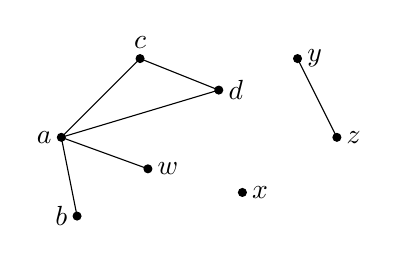
\begin{tikzpicture}
\filldraw (0,0) circle (0.05) node[anchor=east]{$a$};
\filldraw (0.2,-1) circle (0.05) node[anchor=east]{$b$};
\draw (0,0) -- (0.2,-1);
\filldraw (1, 1) circle (0.05) node[anchor=south]{$c$};
\filldraw (2, 0.6) circle (0.05) node[anchor=west]{$d$};
\draw (0,0) -- (1,1); \draw (1,1) -- (2, 0.6); \draw (0,0) -- (2, 0.6);
\filldraw (1.1, -0.4) circle (0.05) node[anchor=west]{$w$};
\draw (0,0) -- (1.1, -0.4);
\filldraw (2.3, -0.7) circle (0.05) node[anchor=west]{$x$};
\filldraw (3,1) circle (0.05) node[anchor=west]{$y$}; \filldraw (3.5,0) circle (0.05) node[anchor=west]{$z$}; \draw (3,1) -- (3.5, 0);
\end{tikzpicture}
\end{center}
For the purposes of this discussion, a \textit{finite graph} is a graph where the set of vertices $V$ is finite. We first state the following definition.
\begin{definition}
Let $G$ be a graph, and let $v$ be a vertex. A \textit{neighbor} of $v$ is a vertex that is connected to $v$ by an edge.
\end{definition}
\begin{example}
In the graph above, $a$ has the neighbors $b, c, d,$ and $w$. Meanwhile, $y$ has one neighbor $z$, and $x$ has no neighbors.
\end{example}

We now state and prove our main theorem, which will demonstrate the pigeonhole principle. Notice that in the graph above, $z$ and $w$ have the same number of neighbors: just one. This is in fact an example of something more general:
\begin{theorem}
Suppose $G$ is a finite graph with at least $2$ vertices. Then there exist $2$ distinct vertices on the graph such that they have the same number of neighbors.
\end{theorem}
\begin{proof}
Suppose $G$ has $n$ vertices, where $n\geq 2$. Thus, if $v$ is a vertex, then $v$ can have \textit{at most} $n-1$ neighbors, as we have disallowed loops in our graphs. Suppose there is some vertex $u$ with the maximum number of neighbors. This means that no vertex can have no neighbors, as $u$ is connected to everything. Similarly, if there is some vertex $w$ with no neighbors, then no vertex can have the maximum number of neighbors $n-1$, as each vertex will miss $w$ as a possible neighbor. Thus, we have two cases:
\begin{enumerate}
    \item Across all vertices, the number of neighbors is in the set $\{0, 1, \ldots, n-2\}$.
    \item Across all vertices, the number of neighbors is in the set $\{1, 2, \ldots, n-1\}$.
\end{enumerate}
However, in each case we have $n$ vertices on our graph, and each vertices has $(n-1)$ possible choices of a number of neighbors to choose from. Hence, it is impossible for each vertex to have a distinct number of neighbors, so there must exist $2$ distinct vertices with the same number of neighbors.
\end{proof}
The end of the argument above demonstrates the pigeonhole principle --- the number of objects we have exceeds the number of choices, so two distinct objects must make the same choice. Alternatively stated in terms of functions:
\begin{theorem}[Pigeonhole Principle]
Let $A, B$ be finite sets, and $f: A\to B$ be a function. If $|A| > |B|$, then $f$ is not injective.
\end{theorem}
This is illustrative of a more general principle:
\begin{theorem}[Functions and Cardinality]
Let $A, B$ be finite sets.
\begin{enumerate}
    \item[$1.$] If there exists an injection $f: A\to B$, then $|A| \leq |B|$.\footnote{This is the contrapositive of the Pigeonhole Principle.}
    \item[$2.$] If there exists a surjection $f: A\to B$, then $|A| \geq |B|$.
    \item[$3.$] If there exists a bijection $f: A\to B$, then $|A| = |B|$.
\end{enumerate}
\end{theorem}
\section{Quantifiers}
We have already seen the words ``for every/all" and ``there exists" in our previous work. These are what are known as \textit{quantifiers} in logic, which we allow ourselves to use when writing complex propositions. First, we introduce some notation. Let $P$ be some statement (usually some property), and $x\in X$ be some object. We write $P(x)$ to mean ``$P$ is true of $x$." Formally, we are defining a function $P: X\to \set{\text{set of propositions}}$.
\begin{example}
Let $P(n)$ be the propositions of the form ``$n$ is even." Then $P(2)$ is true, as $2$ is even, and so is $\lnot P(3)$, as it is not the case that $3$ is even. We can use our familiar logical connectives to deduce that $P(2) \land P(4)$, $P(2)\lor P(-1)$, $P(2) \iff (3 = 3)$, and $P(2) \implies (2+2=4)$ are all logically true statements.
\end{example}
We extend this by defining quantifiers.
\begin{definition}
Let $X$ be a set, and let $P$ be a function $P: X\to \{\text{set of propositions}\}$. We define the following \textit{quantifiers}:
\begin{enumerate}
    \item The \textit{existential quantifier} $\exists$, read ``there exists," is used to assert that there is at least one $x\in X$ such that $P(x)$ is true:
    $$(\exists x\in X)\, P(x) = \text{``there is an } x \text{ such that } P \text{ is true of } x."$$
    \item The \textit{universal quantifier} $\forall$, read ``for every," is used to assert that for every $x\in X$, $P(x)$ is true:
    $$(\forall x\in X)\, P(x) = \text{``for every } x,\, P \text{ is true."}$$
\end{enumerate}
If the set $X$ is clear from context, we write $\exists x$ and $\forall x$ instead of $\exists x\in X$ and $\forall x\in X$.
\end{definition}
 
Quantifiers can be manipulated like the rest of our logical connectives. In particular, they play nicely with our negation operation, which we leave the reader to verify:
\begin{proposition}
Let $P(x)$ be a set of propositions about elements in some set $X$. Then $\lnot \exists x\, P(x) \equiv \forall x\, \lnot P(x)$ and $\lnot \forall x\, P(x) \equiv \exists x\lnot P(x)$.
\end{proposition}
We also stress that the order of quantifiers, when there are many of them, is important. Consider the following example.
\begin{example}
Let us discuss these two statements about positive integers:
\begin{enumerate}
    \item $(\forall m\in \Z^+)\, (\exists n\in\Z^+) \, (m < n)$;
    \item $(\exists n\in\Z^+)\, (\forall m\in\Z^+)\, (m < n)$.
\end{enumerate}
The first of these reads, ``for every positive integer $m$, there exists another positive integer $n$ such that $n$ is greater than $n$," equivalently, ``there is no largest integer." This is evidently true. However, the second of these reads ``there exists a positive integer $n$, such that for every positive integer $m$, we have $m$ is less than $n$," equivalently, ``there \textit{is} a largest integer," which is the negation of statement (1).
\end{example}
Try negating the following statements involving multiple quantifiers:
\begin{exercise}
Find the negation of the following two statements.
\begin{itemize}
    \item[(a)] $(\forall n\in\Z^+)\, (\exists x \in \R)\, (x< 1/n)$;
    \item[(b)] $(\forall x\in\R)\, (\exists y\in \R)\, (xy = 1)$.
\end{itemize}
Which of these two statements is true?
\end{exercise}
\section{Induction I: The Basic Principle}
Now, we turn our attention to the case where $P(n)$ represents some property of positive integers, so we are picking $n\in \Z^+$. Often, we would like to prove a statement of the form $(\forall n\in\Z^+)\, P(n)$; however, it would seem like there is an infinite list of things to check. However, here we introduce the \textit{principle of induction}, which boils down to showing two things.
\begin{theorem}[Induction Principle]
Suppose we would like to prove $(\forall n\in\Z^+) P(n)$. Then it suffices to prove $P(1)$ and $P(n) \implies P(n+1)$ for an arbitrary integer $n$. That is,
$$\Big[P(1) \land \big(P(n)\implies P(n+1)\big)\Big] \implies \forall n\, P(n).$$
\end{theorem}
Intuitively, we have a \textit{base case} $P(1)$ to fall back on, and proving the \textit{inductive step} $P(n)\implies P(n+1)$, where $n$ is \textit{arbitrary}, means we can chain implications together:
$$P(1) \implies P(2), P(2)\implies P(3), P(3)\implies P(4), \ldots,$$
in order to show $P(1) \implies P(n)$ for every $n\in\Z^+$. Since $P(1)$ is true, $P(n)$ must also be true for the implication $P(1)\implies P(n)$ to be true. We view some examples.  
\begin{example}
Prove that for all $n\in\Z^+$, we have $\ds\sum_{k=1}^n k = \frac{n(n+1)}2$.
\end{example}
\begin{proof}
We proceed by induction on $n$. First, we verify that the base case $n=1$ holds: \newpage
$$\sum_{k=1}^1 1 = 1 = \frac{1(1+1)}2.$$
Now, assume the induction hypothesis, that $1+2+ \cdots + n = n(n+1)/2$ for some arbitrary $n$. We compute
$$\sum_{k=1}^{n+1}k = (1 + 2 + \cdots + n) + (n+1) = (n+1) +\sum_{k=1}^n k,$$
so by our induction hypothesis, we have
$$\sum_{k=1}^{n+1} k = (n+1) + \frac{n(n+1)}2 = \frac{(n+1)(n+2)}2,$$
where the reader can check the algebra in this last equality. This completes the proof.
\end{proof}
\begin{example}
Prove that for every $n\geq 1$, we have
$$1\cdot 2 + 2\cdot 3 + \cdots + n(n+1) = \frac 13n (n+1)(n+2).$$
\end{example}
\begin{proof}
We prove by induction on $n$. We verify the base case $n=1$:
$$1\cdot 2 = 2 =  \frac 13(1)(1+1)(1+2) = \frac 13 (2)(3).$$
Now, we assume the inductive hypothesis that $\ds\sum_{k=1}^n k(k+1) = \frac 13n(n+1)(n+2)$ for some arbitrary $n\geq 1$, and we compute
$$\sum_{k=1}^{n+1}k(k+1) = (n+1)(n+2) + \sum_{k=1}^n k(k+1) = (n+1)(n+2) + \frac 13n(n+1)(n+2)$$
$$=(n+1)(n+2)\brak{1 + \frac 13n} = \frac 13(n+1) (n+2) (n+3),$$
which completes the proof.
\end{proof}
The above examples demonstrate an important principle when working with sums: split the sum appropriately. Here is an example with a different flavor.
\begin{example}
Prove that for every $n\in\Z^+$, we have $n + (n+1) + \cdots + 2n = \frac 32n(n+1)$.
\end{example}
\begin{proof}
We prove by induction on $n\in\Z^+$. The base case $n=1$ is easy to verify:
$$1 + 2 = 3 = \frac 32(1)(2).$$
Now, assume that our statement is true for some arbitrary $n\geq 1$. We compute  
$$S:=(n+1) + (n+2) + \cdots + 2(n+1) = [(n+1) + (n+2) + \cdots + 2n] + (2n+1) + (2n+2).$$
The induction hypothesis almost applies, so we make a slight adjustment:
$$S = \brak{\frac 32n(n+1) - n} + (4n+3) = \frac 32n(n+1) + 3n+3 = \frac 32n^2 + \frac 32n + 3n+3$$
$$=\frac 32n^2 + \frac 92n + 3 = \frac 32(n^2 + 3n+2) = \frac 32(n+1)(n+2),$$
so we are done.
\end{proof}
Induction can be used to prove more than just sums:
\begin{example}
Prove that for any $n\in\Z$, $n^5-n$ is a multiple of $5$.
\end{example}
\begin{proof}
We first take the case where $n\geq 0$. Here, we apply induction on all non-negative $n$. Our base case starts at $n=0$, and we see that $0^5-0 = 0$, which is a multiple of $5$. Now, suppose that $n^5-n$ is a multiple of $5$, where $n\geq 0$ is arbitrary. Then
$$(n+1)^5-(n+1) = (n^5+5n^4+10n^3+10n^2+10n+1) - n-1$$
$$=(n^5-n) + 5(n^4+2n^3+2n^2+n).$$
The first of these terms is divisible by $5$ by the induction hypothesis, and the second of these terms is obviously divisible by $5$. Hence, we are done when $n\geq 0$.

If $n\leq 0$, note that $-n\geq 0$, so that $(-n)^5 - (-n) = -(n^5-n)$ is divisible by $5$ by our previous case. Flipping signs gives us what we need, so we are done for all $n\in\Z$.
\end{proof}
\begin{example}
Prove that for all $n\in\Z^+$, we have $4^n < (n+2)!$.
\end{example}
\begin{proof}
We prove by induction on $n\in\Z^+$. For the base case $n=1$, we have $4^1 = 4 < 6 = (1+2)!$. Assume that $4^n < (n+2)!$ for an arbitrary $n\in\Z^+$. Then
$$4^{n+1} = 4\cdot 4^n < 4 \cdot (n+1)!$$
by the induction hypothesis, but now since $n \geq 1$, we must have $n+3\geq 4$, so we may replace and write
$$4^{n+1} < 4\cdot (n+1)! \leq (n+3)(n+2)! = (n+3)! = [(n+2)+1]!,$$
so by induction, we are done.
\end{proof}
We leave these exercises for the reader to try.
\begin{exercise}
Prove that every finite subset of $\R$ has a minimum element.
\end{exercise}
\begin{exercise}
Show that for all positive integers, we have $$\sum_{k=0}^{n} q^k = \frac{q^{n+1}-1}{q-1}$$
as long as $q\neq 1$.
\end{exercise}
 
\begin{exercise}
{Show that the sum of the first} $n$ {odd positive integers is} $n^2$, {more precisely} that
$$n^2 = \sum_{k=1}^{n} (2k-1) \textrm{ for all } n\in \Z^+.$$
\end{exercise}
\begin{exercise}
Prove that for all $n\in\Z^+$, we have $2^n + n \leq 3^n$.
\end{exercise}
\begin{exercise}
The \textit{gamma function} $\Gamma: (0, \infty) \to \R$ is defined by
$$\Gamma(x) := \int_0^\infty t^{s-1}e^{-t}\, dt.$$
Show that $\Gamma(n) = (n-1)!$ for every $n\geq 1$.
\end{exercise}
\section{Induction II: Strong Induction}
Sometimes, induction is not enough to prove a statement of the form $(\forall n\in\Z^+)\, P(n)$, due to the way the problem requires more assumptions. However, there is a (relatively) easy fix: just assume more assumptions when we do the induction step.
\begin{theorem}[Strong Induction Principle]
Suppose we would like to prove $(\forall n\in\Z^+) P(n)$. Then it suffices to prove $P(1)$, and that $[P(1) \land P(2) \land \cdots \land P(n)] \implies P(n+1)$.
\end{theorem}
That is, we show $P(1)$, and we assume the statements $P(k)$ are all true for all $1\leq k \leq n$, from which we deduce $P(n+1)$. We view an example, which is an important theorem we will use later on.
\begin{theorem}[Fundamental Theorem of Arithmetic] \label{fundamental theorem of arithmetic}
Every natural number $n\geq 2$ can be factored into primes, and this factorization is unique up to changing the order of the factors.    
\end{theorem}
We will prove existence via strong induction.
\begin{proof}[Proof of Existence of Factorization]
We check our base case $n=2$: the number $2$ is prime, so our factorization is simply $2 = 2$. Now, assume the strong induction hypothesis that every integer $k$, with $2\leq k \leq n$, can be factored as a product of primes. Consider the integer $n+1$. If $n+1$ is prime, then $n+1 = n+1$ is a factorization into primes. Otherwise, $n+1$ is composite and there exist integers $a,b$ with $2 < a,b < n+1$ such that $n+1 = ab$. By the inductive hypothesis, factor both $a$ and $b$ into primes:
$$a = p_1p_2\cdots p_m, b = q_1q_2\cdots q_\ell,$$
where the $q_i$'s and $q_j$'s are all prime. Hence
$$n+1 = (p_1p_2\cdots p_m)(q_1q_2\cdots q_\ell) = \prod_{i=1}^m p_i \prod_{j=1}^\ell q_j$$
is a factorization of $n+1$ into primes.
\end{proof}
Notice that the strong induction hypothesis was actually necessary here: we did not know \textit{exactly} what $a$ and $b$ were, only that they were in the range to apply the strong induction hypothesis on.

Strong induction is often used when we have a \textit{recursive} definition of a sequence $f: \Z^+ \to X$. One prototypical example of this is the Fibonacci sequence:
\begin{definition}\label{fibonacci}
The \textit{Fibonacci sequence} is the function $F: \Z^+ \to \Z^+$ defined as follows: $F(1) = F(2) = 1$, and $F(n) = F(n-1) + F(n-2)$ for every $n\geq 3$.
\end{definition}
We often write $F_n$ in place of $F(n)$ for sequences such as this one.
\newpage
\begin{example}
For every $n\in\Z^+$, define $S_n$ to be the set of sequences of $1$'s and $2$'s that sum to $n$. For example, $S_1 = \{(1)\}$, $S_2 = \{(2), (1, 1)\}$, and $S_3 = \{(1,1,1), (1,2), (2,1)\}$. Show that $|S_n| = F_{n+1}$ for every $n\in\Z^+$.
\end{example}
\begin{proof}
We prove by strong induction. Here, we need to check two base cases, due to how the Fibonacci sequence is defined. Clearly, the example above shows that $|S_1| = 1 = F_2$ and $|S_2| = 2 = F_3$, so the base cases hold. Now, assume $n\geq 3$, and that the induction hypothesis holds for all $k < n$. [Note that this is simply a different way of phrasing the induction step in strong induction.] Let $(s_1, \ldots, s_k)$ be a sequence of $1$'s and $2$'s that sum to $n$. If $s_1 = 1$, then the subsequence $(s_2, \ldots, s_k)$ sums to $n-1$; similarly, if $s_1 = 2$, then the subsequence $(s_2, \ldots, s_k)$ sums to $n-2$. Alternatively stated, every sequence in $S_n$ is of the form $(1, s_2, \ldots, s_k)$ or $(2, t_2, \ldots, t_k)$, where $(s_2, \ldots, s_k)\in S_{n-1}$ and $(t_2, \ldots, t_k)\in S_{n-2}$. By counting and the induction hypothesis, we see that $|S_n| = |S_{n-1}| + |S_{n-2}| = F_n + F_{n-1} = F_{n+1}$.
\end{proof}

\begin{example}
We show that any $k\in\Z^+$ has a \textit{binary expansion}: i.e., for every $k\in\Z^+$, there exist integers $0 \leq k_1 < k_2 < \cdots < k_\ell$ such that $n = 2^{k_1} + 2^{k_2} + \cdots + 2^{k_\ell}$.
\end{example}
\begin{proof}
We prove by strong induction. The base case $n=1$ is simple enough: $1 = 2^0$. Now, assume for some $k\geq 1$, the statement holds for all integers less than or equal to $k$. Let $n := k+1$. Let $j\in \N$ be such that $2^j \leq n$ but $2^{j+1} > n$; that is, $j := \floor{\log_2 n}$, and set $m := n - 2^j$. Clearly, $m\geq 0$. If $m = 0$, then $n = 2^j$ and we are done.

In the case that $m > 0$, we note that $m = n-2^j = j+1 - 2^j \leq k+1 - 1 = k$, so the induction hypothesis applies, so there exist $0 \leq k_1 < k_2 < \cdots < k_\ell$, all integers, such that $m = 2^{k_1} + \cdots + 2^{k_\ell}$. We make the claim that $j\neq k_i$ for any $i = 1, 2, \ldots, \ell$. Otherwise, if $j=k_i$ for some $k_i$, we would have $n = m + 2^j = m+2^{k_i}  = (2^{k_1} + \cdots + 2^{k_i} + \cdots + 2^{k_\ell}) + 2^{k_i} \geq 2\cdot 2^{k_i} = 2^{k_i+1} = 2^{j+1}$, but this would contradict our definition of $j$. Thus
$$n = m+2^j = 2^{k_1} + 2^{k_2} + \cdots + 2^{k_\ell} + 2^{j},$$
where each integer is distinct. Now, put the integers $j, k_1, k_2, \ldots, k_\ell$ in order to complete the proof.
\end{proof}
Here are two strong induction exercises.
\begin{exercise}
Let $a_1 = 3/2$, $a_2 = 7/12$ and $6a_{k+2} =5 a_{k+1}-a_k$ for all $k\geq 1$. Prove that
$$a_k = \frac 1{2^k} + \frac 1{3^{k-1}}.$$
\end{exercise}
\begin{exercise}
Let $x_1=2$, $x_2=12$ and for any positive integer $n$, define $x_{n+2} = 2x_{n+1}+4x_n$. Show that $x^n$ is a multiple of $2^n$ for all $n$.
\end{exercise}
\section{Induction III: The Binomial Coefficient}
One particular function often arises in combinatorics, but also in other unexpected areas. In this section, we explore the \textit{binomial coefficient} and its relationship to induction.
\begin{definition}
Let $n,k\in \Z_{\geq 0}$, with $k\leq n$. We define the \textit{binomial coefficient} $\binom nk$ by $\binom n0 = 1 = \binom nn$ if $k= 0, n$, and recursively by $\binom nk = \binom{n-1}k + \binom{n-1}{k-1}$ otherwise.
\end{definition}
\newpage
For us, binomial coefficients have one major interpretation.
\begin{proposition}
There are $\binom nk$ subsets of cardinality $k$ of $\{1, 2, \ldots, n\}$.
\end{proposition}
\begin{proof}
We apply a ``double induction" on $n$ and $k$. In the case that $k=0$ or $k=n$, this is obvious: there is one subset of zero elements ($\varnothing$) and one subset containing $n$ elements (the whole set). Of course, we have $\binom n0 = \binom nn = 1$. For the inductive step, suppose $1\leq k \leq n-1$ and suppose $\binom mj$ is the number of $j$-element subsets of an $m$-element set, whenever $j<k$ or $m<n$. Consider a $k$-element subset of $\{1, 2, \ldots, n\}$; call this subset $X$. We consider two disjoint cases.

\textit{Case I:} $1\not\in X$. In this case, $X \subseteq \{2, 3, \ldots,n\}$, which is a set of $n-1$ elements. Apply the inductive hypothesis, and there are such $\binom{n-1}k$ sets of size $k$ inside $\{2, 3, \ldots, n\}$.

\textit{Case II:} $1\in X$. In this case, let $Y := X\setminus\{1\}$. Then $|Y| = k-1$, and $Y\subseteq \{2, \ldots, n\}$. By induction, there are $\binom{n-1}{k-1}$ such sets.

Now, adding together the disjoint cases, we have $\binom {n-1}k + \binom{n-1}{k-1} = \binom nk$ such $k$-element subsets of $\{1, 2, \ldots, n\}$.
\end{proof}

Next, we prove an important theorem from algebra, using induction.
\begin{theorem}[Binomial Theorem]\label{binomial theorem}
For all $x,y\in\C$ and $n\in \Z^+$, we have
$$(x+y)^n = \sum_{k=0}^n \binom nk x^{n-k}y^k.$$
\end{theorem}
\begin{proof}
We prove by induction on $n$. The base case $n=1$ is easy to verify: $(x+y)^1 = x+y = \binom 10 x + \binom 11 y$. Now, suppose the theorem holds for some $n \geq 1$. We expand $(x+y)^{n+1}$:
\begin{align}
    (x+y)^{n+1} &= (x+y)(x+y)^n \\
    &= (x+y)\brak{\sum_{k=0}^n \binom nkx^{n-k}y^k} \label{binom ind} \\
    &= x\brak{\sum_{k=0}^n \binom nkx^{n-k}y^k} + y \brak{\sum_{k=0}^n \binom nkx^{n-k}y^k} \\
    &= \brak{x^{n+1}+\binom n1x^ny +\cdots  + xy^n}  +\brak{x^ny + \binom n1 x^{n-1}y^2 +\cdots+ y^{n+1}} \\
    &= x^{n+1} + \brak{\binom n0 + \binom n1}x^ny + \brak{\binom n1+\binom n2}x^{n-1}y^2 + \cdots + y^{n+1} \\
    &= \binom{n+1}0 x^{n+1} + \binom{n+1}1 x^ny + \binom{n+1}x^{n-1}y^2 + \cdots + \binom{n+1}{n+1}y^{n+1}, \label{binom def pf}
    \end{align}
where \eqref{binom ind} comes from the inductive hypothesis and \eqref{binom def pf} comes from the definition of the binomial coefficient. This completes the proof.
\end{proof}

Next, we give some examples of manipulating the binomial coefficient effectively.
\begin{example}
We claim that $\ds\sum_{k=0}^n \binom nk = 2^n$.
\end{example}
\begin{proof}
We prove by induction on $n$. The base case $n=1$ is obvious: $\sum_{k=0}^1 \binom 1k = \binom 10 + \binom 11 = 1+1=2=2^1$. Now, suppose the claim holds for some $n\geq 1$. Then we expand:
\newpage
We have, noting that $\binom j0 = \binom jj = 1$ for all $j\in\Z^+$,
\begin{align*}
    \sum_{k=0}^{n+1}\binom{n+1}k &= \binom{n+1}0 + \binom{n+1}1 + \cdots + \binom{n+1}n + \binom{n+1}{n+1} \\
    &= \binom n0 + \brak{\binom n0 + \binom n1} + \cdots + \brak{\binom{n}{n-1} + \binom nn} + \binom nn \\
    &= 2\binom n0 + 2\binom n1 + \cdots + 2\binom n{n-1} + 2\binom nn = 2\sum_{k=0}^{n}\binom nk,
\end{align*}
For the second step, we used the definition of the binomial coefficient. Now, the inductive step finishes the proof:
$$\sum_{k=0}^{n+1} \binom{n+1}k = 2\sum_{k=0}^n \binom nk = 2\cdot 2^n = 2^{n+1},$$
so we are done.
\end{proof}
\begin{exercise}
Give an alternative proof of the above example by appealing to Theorem \ref{power set size}.
\end{exercise}

Our final example relates our definition of the binomial coefficient to a common alternate definition often used by textbooks.
\begin{proposition}\label{factorial formula for binom}
For all $n, k\in \Z_{\geq 0}$ with $n \geq k$, we have $\ds\binom nk = \frac{n!}{k!(n-k)!}$.
\end{proposition}
\begin{proof}
We prove by ``double induction" on $n$ and $k$. We check two base cases: $\binom n0 = 1 = n!/(n! \cdot 0!) = \binom nn$. For the induction hypothesis, assume that
$$\binom mj = \frac{m!}{j!(n-j)!}$$
for all $m<n$ and $j<k$. Now
\begin{align*}
\binom nk = \binom{n-1}k + \binom{n-1}{k-1} &= \frac{(n-1)!}{k!(n-1-k)!} + \frac{(n-1)!}{(k-1)!(n-k)!} \\
&= \frac{(n-1)!}{k!(n-k-1)!} \cdot \frac{n-k}{n-k} + \frac{(n-1)!}{(k-1)!(n-k)!} \cdot \frac kk \\
&= \frac{(n-1)! (n-k) + (n-1)!k}{k!(n-k)!} = \frac{(n-1)!(n-k+k)}{k!(n-k)!} \\
&= \frac{n!}{k!(n-k)!},
\end{align*}
which completes the proof.
\end{proof}
Here are some slightly more interesting examples for the reader to solve.
\begin{exercise}
Let $0\leq k\leq m\leq n$. Show that $\ds\binom mk\binom nm = \binom nk\binom{n-k}{m-k}$.
\end{exercise}
\begin{exercise}
Let $n\geq 1$. Show that $\ds\binom n0-\binom n1 + \binom n2 - \cdots + (-1)^n\binom nn = 0$.
\end{exercise}
\begin{exercise}
Let $n\geq 1$. Show that $\ds\sum_{k=1}^n k\binom nk = n2^{n-1}$.
\end{exercise}
\begin{exercise}
Let $n\geq 1$. Show that $\ds\sum_{k=1}^n k(-1)^k 2^{n-k}\binom nk = -n$.
\end{exercise}
\begin{exercise}
Using the fact that $(1+x)^n(1+x)^n = (1+x)^{2n}$, show that
$$\sum_{r=0}^k \binom nr\binom n{k-r} = \binom{2n} k.$$
\end{exercise}
\section{Divisibility I: Basic Principles}
We now move into the number theory part of Math 13. A lot of number theory is based on the idea of \textit{divisibility}, which we will discuss later, but first, let us consider a special case: divisibility by $2$.
\begin{definition}
Let $n\in \Z$.\footnote{We again remind the reader that $\Z$ denotes the integers. We will be seeing a lot of $\Z$'s in this part of the course.} We say that $n$ is \textit{even} if $n = 2k$ for some $k\in \Z$. Similarly, we say that $n$ is \textit{odd} if $n = 2k+1$ for some $k\in\Z$.
\end{definition}
Alternatively worded, $n$ is even if it is ``divisible by $2$," whatever that means. We first note an obvious-sounding property of evenness and oddness, which will have important ramifications later --- which is to say, do not skip this proof!
\begin{proposition}
Every integer is either even or odd, and no integer is both even and odd.
\end{proposition}
\begin{proof}
We first prove the statement that every integer is either even or odd. Let $n\in \Z$. We need only consider the non-negative integers, as we can just ``flip" things around for negative integers. Hence, we apply induction on all $n \geq 0$. The base case $n=0$ is obvious: $0 = 2\cdot 0$, so $0$ is even. Now, suppose that $n$ is either even or odd, for some $n \geq 0$. We consider $2$ cases.

\textit{Case I:} $n$ is even. Then $n = 2k$ for some $k\in\Z$. But then $n+1 = 2k+1$, so $n+1$ is odd.

\textit{Case II:} $n$ is odd. Then $n = 2j+1$ for some $j\in\Z$. But then $n+1 = 2j+2 = 2(j+1)$. Letting $m := j+1$, we see $n+1 = 2m$, so $n+1$ is even.

Thus, every integer (reflecting this for negative integers) is either even or odd.

Now, we show that no integer is both even and odd. Suppose for contradiction that $n\in\Z$ is both even and odd. Then $n = 2k$ and $n = 2j+1$ for $j,k\in\Z$.\footnote{Notice that we really need two distinct variables here!} Thus, $n = 2k = 2j+1$, which implies $2(k-j) = 1 \iff k-j = 1/2$. But since $k, j\in \Z$, we have $1/2\in \Z$, which is impossible. Hence, no integer is both even and odd.
\end{proof}

We now take a look at the more general notion of divisibility by any number. \newpage

\begin{definition}\label{divisibility}
Let $m,n\in\Z$. We say that $m$ \textit{divides} $n$ if there exists a $k\in \Z$ such that $n = km$. We write $m\mid n$ when $m$ divides $n$, and $m\nmid n$ otherwise.
\end{definition}

This allows us to rewrite the definition of an even integer: $n$ is even if and only if $2 \mid n$.

\subsection*{Grade-School Division}
Recall the type of division we learned in $3$rd grade prior to learning about fractions --- given a number, say $27$ apples, we wanted to know how we can split that evenly amongst, say $5$ friends. Clearly, each friend gets $5$ apples, with $2$ leftover --- that is, our division had a quotient and remainder. It is this sort of division that we will interest ourselves with for the rest of the course.

\begin{theorem}[Division Algorithm]
Let $k\geq 2$ be an integer. For any $n\in\Z$, there exist $q\in\N$ and $r\in\{0, 1, \ldots, k-1\}$, both unique, such that $n = qk + r$.
\end{theorem}
That is to say, the quotient and remainder from grade-school are always unique --- intuitively, we know this to be true, but let us see the proof.
\begin{proof}
We first prove the existence of $q$ and $r$. Fix $k\geq 2$, and we apply induction on non-negative $n\in\Z$. [Of course, we flip everything around as necessary when $n<0$.] For $n=0$, we simply set $q=r=0$. Now, assume the inductive hypothesis, and $n = kq+r$ for $q\in\Z$ and $r\in\{0, 1, \ldots, k-1\}$. We then see that $n+1 = kq + r+1$, and we consider $2$ cases.

\textit{Case I:} $r < k-1$. In this case, there is nothing to do, simply set $q' = q$ and $r' = r+1$. Notice that $r' \in \{0, 1, \ldots, k-1\}$ in this case, so this is legal. Hence $n+1 = q'k + r'$.

\textit{Case II:} $r = k-1$. Then $n+1 = kq + r+1 = kq + (k-1)+1 = k(q+1)$. Hence, set $r'=0$ and $q' = q+1$, so $n+1 = q'k + r'$.

Now, we prove uniqueness. Fixing $k\geq 2$ and some $n\in\Z$, suppose $n = qk+r = q'k+r'$ for $q, q'\in \Z$ and $r, r' \in \{0, 1, \ldots, k-1\}$. It suffices to show $q=q'$ and $r=r'$. 

First, we have $n = qk+r = q'k + r'$. By some algebra, we write this as $k(q - q') = r'-r$. Since $q-q'$ is an integer, we see by the definition of divisibility that $k\mid (r'-r)$. Without loss of generality, assume $r'\geq r$. But then $r',r \in \{0, 1, \ldots, k-1\}$ implies $r'-r \in \{0, 1, \ldots, k-1\}$, so the divisibility condition is impossible unless $r' = r$.

From the fact that $r'=r$, we simply have $qk + r = q'k + r' \implies qk = q'k \implies q=q'$, so we are done.
\end{proof}
Notice that the assumption that $r$ was taken from $\{0, 1, \ldots, k-1\}$ is very important!
\begin{exercise}
Replace $r\in\{0,1, \ldots, k-1\}$ from the statement of the Division Algorithm with $r\in\Z$. Give a counterexample to show that uniqueness fails.
\end{exercise}
With the Division Algorithm in place, we now show that our way of writing numerics makes sense. For example, the number $123$ is literally a string of digits, but we take this to mean
$$123 = 1 \times 10^2 + 2\times 10^1 + 3\times 10^0.$$
In fact, the representation of this number is unique in base $10$, as the following theorem shows.
\begin{theorem}\label{base d expansion}
For any $n\geq 1$ and $k\geq 2$, there exist unique $r\in\Z^+$ and $d_0, d_1, \ldots, d_r \in\{0, 1, \ldots k-1\}$ such that $n = d_rk^r + d_{r-1}k^{r-1} + \cdots +d_1k + d_0$ and $d_r \neq 0$.
\end{theorem}
Taking $k=10$, this simply says a number can be written uniquely in base $10$. We prove existence and leave uniqueness to the reader. \newpage

\begin{proof}[Proof (of existence)]
We apply strong induction on $n\geq 1$. For our base case, we check $n$ satisfying $1 \leq n \leq k-1$. In this case, we take $r=0$ and $d_0 = n$.

Now, assume the inductive hypothesis, that the theorem holds for all $\ell < n$, where $n\geq 1$ is some integer. Now, we apply the Division Algorithm to $n$ to write $n = kq + d_0$, where $d_0\in\{0, 1, \ldots, k-1\}$. Suppose $n\geq k$, so $q\geq 1$. We apply the inductive hypothesis on $q$: write
$$q = d_rk^{r-1} + d_{r-1}k^{r-2} + \cdots + d_2k + d_1,$$
for appropriate $d_1, \ldots, d_r\in \{0,1, \ldots, k-1\}$ and $d_r \neq 0$. Hence
$$n = kq + d_0 = k(d_r k^{r-1} + d_{r-1}k^{r-2} + \cdots + d_2k + d_1) + d_0$$
$$=d_rk^r + d_{r-1}k^{r-1} + \cdots + d_2k^2 + d_1k + d_0,$$
as expected.
\end{proof}
\begin{exercise}
The uniqueness proof is hidden inside the existence proof above. Rephrase the proof to account for uniqueness.
\end{exercise}

\subsection*{Modular Arithmetic}
The division algorithm also justifies another important construction, which allows us to tell the time. In a 12-hour system, we say that $5$ hours after 9:00 is not 14:00, but rather 2:00. In some sense, the clock ``wraps around" after 12:00. We generalize this into \textit{modular arithmetic}, which is ubiquitous across most of abstract algebra.
\begin{definition}
Let $k\geq 2$, and let $n\in\Z$, so by the Division Algorithm we write $n = kq+r$ for $r\in\{0, 1, \ldots, k-1\}$. The \textit{remainder of $n$ modulo $k$} is the number $r$, and we say that $m,n\in\Z$ are \textit{congruent modulo $k$} if they have the same remainder modulo $k$.
\end{definition}
Notice that we are justified in saying \textbf{the} remainder due to the uniqueness condition of the Division Algorithm. In speech, we often abbreviate ``modulo" by simply saying ``mod"; hence we write $m\equiv n\pmod k$ to mean $m$ and $n$ are congruent modulo $k$. Of course, when $k$ is clear from context, we will be lazy and say ``$m$ and $n$ are congruent."
\begin{example}
Let $k=10$. Then $m\equiv n\pmod{10}$ if and only if $m$ and $n$ have the same last digit: e.g., $17 \equiv 7\pmod{10}$. The reason for this follows from Theorem \ref{base d expansion}.
\end{example}

\begin{example}
Let $k=2$. Then $n\equiv 0$ if and only if $n$ is even, and $n\equiv 1$ if and only if $n$ is odd.
\end{example}

The two following propositions are very important.
\begin{proposition}\label{mod div}
Let $k\geq 2$, and let $m,n\in\Z$. Then $m\equiv n\pmod k$ if and only if $k\mid(m-n)$. In particular, $n\equiv 0\pmod k$ if and only if $k\mid n$.
\end{proposition}
\begin{proof}
$(\implies)$: Suppose $m\equiv n\pmod k$. Then $m = q_1k+r$ and $n = q_2k + r$ for $r\in\{0, 1, \ldots, k-1\}$ and $q_1,q_2\in \Z$. Now $m-n = q_1k - q_2k = k(q_1 - q_2)$, which is a multiple of $k$.

$(\impliedby)$: Suppose $k\mid (m-n)$. Write $m = q_1k + r_1$ and $n = q_2k + r_2$ by the Division Algorithm. Now $m-n = (q_1 - q_2)k + (r_1 - r_2)$. Since $k\mid (m-n)$, we have $k \mid (r_1 - r_2)$, but by the fact we chose $r_1, r_2 \in \{0, 1, \ldots, k-1\}$ by the Division Algorithm, we must have $r_1 - r_2 = 0$. Hence $r_1 = r_2$, so that $m\equiv n\pmod k$.  
\end{proof}

\newpage
\begin{proposition}
Let $k\geq 2$. Suppose $m\equiv m'$ and $n\equiv n' \pmod k$. Then $m+n \equiv m' + n'$ and $mn \equiv m'n' \pmod k$.
\end{proposition}
\begin{exercise}
Prove the above proposition.
\end{exercise}
\begin{example}
Let $k=10$. Then $13 + 202 \equiv 3+2 = 5 \pmod{10}$. Similarly, $2\cdot 13 \equiv 2\cdot 6 \pmod{10}$.
\end{example}

Here is an interesting example: the divisibility rule for $3$. Notice that this \textit{only} works if we are in base $10$.
\begin{proposition}[Divisibility Rule for $3$]
Let $n\in\Z_{\geq 0}$. Then $3\mid n$ if and only if the sum of the digits of $n$ is also divisible by $3$.
\end{proposition}
\begin{proof}
By Theorem \ref{base d expansion}, write $n = d_r(10)^r + d_{r-1}(10)^{r-1} + \cdots d_1(10) + d_0$. Now, by the previous proposition, we see that $10 \equiv 1 \pmod 3$, so that $10^j \equiv 1^j = 1\pmod 3$ for any $j\in\Z^+$. Hence, the above reduces to
$$n \equiv d_r(1)^k + d_{r-1}(1)^{k-1} + \cdots + d_1(1) + d_0 \pmod 3$$
$$\implies n\equiv d_r + d_{r-1} + \cdots + d_1 + d_0 \pmod 3,$$
hence $n$ is congruent to the sum of its digits in base $10$, modulo $3$. Now, Proposition \ref{mod div} finishes the proof.
\end{proof}

We end with some exercises.
\begin{exercise}
Prove for any $n\in\Z^+$, we have $7\mid (5^{2n} + 3\cdot 2^{5n-2})$.
\end{exercise}
\begin{exercise}
Prove that $25\mid (4^{200}-1)$.
\end{exercise}
\begin{exercise}
Find the remainder of $1^5 + 2^5 + \cdots + 2022^5$ when divided by $4$.
\end{exercise}

\section{Divisibility II: Common Divisors}
We start with a definition.
\begin{definition}\label{gcd}
Let $m, n\in\Z$. The \textit{greatest common divisor} (GCD) of $m$ and $n$ is the largest $d\in \Z^+$ such that $d\mid m$ and $d\mid n$. We denote the GCD of $m$ and $n$ by $\gcd(m, n)$.
\end{definition}
We note that some algebra texts simply write ``$(m, n)$" for the GCD of $m$ and $n$. Alternatively stating the definition, $d_0 = \gcd(m, n)$ if and only if the following conditional holds:
\begin{center}
If $d\mid m$ and $d\mid n$, then $d\leq d_0$.
\end{center}
We view some examples.
\begin{example}
We have $\gcd(24, 21) = 3$, as $24 = 2^3\times 3$ and $21 = 3\times 7$. Similarly, $\gcd(36, 54) = 2\times 3^2 = 18$, as $36 = 2^2\times 3^2$ and $54 = 2\times 3^3$.
\end{example}
\begin{example}
Let $p, q$ be distinct prime numbers. Then $\gcd(p, q) = 1$ by their primality, as expected. However, the converse is not true: $\gcd(25, 49) = 1$, but neither $25$ nor $49$ are prime. However, this does suggest to us the following definition.
\end{example}
\begin{definition}
Let $m,n\in\Z$. We say $m,n$ are \textit{relatively prime} (or \textit{coprime}) if $\gcd(m, n) = 1$; that is, they have no common prime factors.
\end{definition}

Hence, the previous example tells us that any two prime numbers are coprime, but composite numbers can form coprime pairs as well.
\newpage
\subsection*{Bezout's Lemma}
Consider the following equation of a line: $ax + by = c$, where $a,b,c\in\Z$. In applications, we often care about whether this line passes through a \textit{lattice point}, i.e., a point in the $xy$-plane where both coordinates are integers. Let us consider two exmaples firsts, before we develop the theory.

\begin{example}
Does $2x+6y = 5$ pass through any lattice points?
\end{example}
\begin{solution}
No: notice we can write $5 = 2x+6y = 2(x+3y)$. If $(x,y)$ is a lattice point on the line, then we must that $5$ is an integer multiple of $2$; i.e., $5$ is even. This is impossible.
\end{solution}

\begin{example}
Does $23x + 24y = 17$ pass through any lattice points?
\end{example}
\begin{solution}
Yes, easily: first notice that $23(-1) + 24(1) = 1$. Now, multiplying by $17$ gives the desired result: $(-17, 17)$ sits on the line.
\end{solution}

For the first of these examples, notice that the coefficients $a=2$ and $b=6$ satisfied $\gcd(a,b) = 2$, which ended up showing up in our proof of impossibility. On the other hand, in the second example, $\gcd(a = 23, b=24) = 1$, which nicely divides $17$ (obviously) and thus gave us a lattice point. Hence, the GCD is closely related with the lattice point problem. While comparing prime factors is easy for computing the GCD for small numbers, it falls off quickly as factorization becomes increasingly more difficult for larger numbers. However, we introduce an efficient method to find the GCD, which does not involve factorization, only long division, which is far less expensive.
\begin{theorem}[Euclidean Algorithm]\label{euclidean algorithm}
Suppose $a,b\in\Z^+$ and $a\geq b$. Then this algorithm gives the $\gcd(a, b)$ when it terminates:
\begin{enumerate}
    \item[$(1)$] Firstly, if $a=b$, then clearly $\gcd(a, b) = a=b$.
    \item[$(2)$] Otherwise, use the Division Algorithm to write $a = q_0b + r_0$, for some $q\in\Z^+$ and $r_0 \in \set{0, 1, \ldots, b-1}$. If $r_0 = 0$, then the algorithm terminates and $\gcd(a,b) = b$.
    \item[$(3)$] Else if $r_0 > 0$, find $q_1, r_1$ by the Division Algorithm with $b = q_1r_0 + r_1$. If $r_1 = 0$, then $\gcd(a, b) = r_0$.
    \item[] ...
    \item[$(k+2)$] Else if $r_k > 0$, find $q_{k+1}, r_{k+1}$ by the Division Algorithm with $r_{k-1} = q_{k+1}r_k + r_{k+1}$...
\end{enumerate}
At the point of termination, we have $\gcd(a, b) = r_j$, where $j$ is the last index $k$ such that $r_k > 0$.
\end{theorem}
The proof of the Euclidean algorithm is left in the official Math 13 notes, Exercise 4.2.8, and of course, the algorithm could be used for negative integers in the obvious way. Hopefully, these examples are convincing enough to show that this theorem holds.
\begin{example}
We compute $\gcd(32, 60)$. Setting $a = 60$ and $b = 32$, we write
\begin{align*}
    60 &= 1\cdot \textbf{32} + 28 \\
    32 &= 1\cdot \textbf{28} + 4 \\
    28 &= 7\cdot \textbf{4} + 0.
\end{align*}
Hence $\gcd(60, 32) = 4$.
\end{example}
\newpage
\begin{example}
We compute $\gcd(657, 306)$. Setting $a=657$ and $b = 306$, we write
\begin{align*}
657 &= 2\cdot 306 + 45\\
306 &= 6\cdot 45 + 36 \\
45 &= 1\cdot 36 + 9 \\
36 &= 4\cdot 9 + 0.
\end{align*}
Hence $\gcd(657, 306) = 9$.
\end{example}

It turns out that the solution to our lattice point problem is a corollary of this GCD-finding technique.
\begin{theorem}[Bezout's Lemma]
Let $a,b,c\in \Z$. Then there exist $x,y\in\Z$ such that $ax + by = c$ if and only if $\gcd(a,b) \mid c$.
\end{theorem}
\begin{proof}
$(\implies)$: Suppose for contradiction that there exist $x,y\in\Z$ such that $ax+by= c$, yet $\gcd(a,b) \nmid c$. Since $\gcd(a,b)\mid a,b$ by definition, we have $\gcd(a,b)\mid (ax + by)$, but $c=ax+by$, a contradiction.

$(\impliedby)$: Use the Euclidean algorithm to find $\gcd(a,b) = r_j$ for the integers $r_0, r_1, \ldots, r_j$. Notice that each $r_i$ is a linear combination of $a$'s and $b$'s, so ``reversing" the algorithm as appropriate\footnote{See Math 13 official notes, p. 120-121.} allows us to find $x',y'\in \Z$ such that $\gcd(a,b) = ax'+by'$. Since $\gcd(a,b)\mid c$, multiplying through by $c/\gcd(a,b)$ finishes the proof.
\end{proof}

If this proof was unsatisfying, see the exercises at the end of this section for a different proof. We now give important corollaries of Bezout's Lemma.

\begin{corollary}
Let $a,b\in\Z$. Then $a,b$ are coprime if and only if there exist $x,y\in\Z$ such that $1 = ax+by$.
\end{corollary}
\begin{proof}
$(\implies)$: This follows from Bezout's Lemma with $\gcd(a,b) = 1$.

$(\impliedby)$: Let $d = \gcd(a,b)$. Suppose there exist $x,y\in\Z$ with $1 = ax + by$. Then $d|a$ and $d|b$, so that $a = dm$ and $b=dn$ for some $m,n \in\Z$. Hence $1 = dmx + dny = d(mx + ny)$, so that $1$ is a multiple of $d$. Hence $d=1$; i.e., $\gcd(a,b) = 1$.
\end{proof}

\begin{corollary}\label{euclid1}
Let $a,b,c\in\Z$. If $a \mid bc$ and $a,b$ are coprime, then $a\mid c$.
\end{corollary}
\begin{proof}
Suppose $a\mid bc$ and $a,b$ are coprime. By the previous corollary, there exist $x,y\in\Z$ such that $1 = ax + by$, so that $c = acx + bcy$. However, $a\mid bc$, so $bc = an$ for some $n\in\Z$. It follows that $c = acx  +bcy = acx + y\cdot an = a(cn + ny)$, so $a\mid c$.
\end{proof}
In particular, we get these results when $a$ is prime in the corollary above.
\begin{proposition}
Let $p$ be prime, and let $a\in\Z$. Then $\gcd(a, p) = 1$ if and only if $p\nmid a$.
\end{proposition}
\begin{proof}
We know that $\gcd(a, p) \mid p$. But $p$ is prime, so either $\gcd(a,p) = 1$ or $\gcd(a, p) = p$. The proposition easily follows from this.
\end{proof}

\begin{theorem}[Euclid's Lemma]\label{euclid's lemma}
Let $p$ be prime, and $a,b\in\Z$. If $p\mid ab$, then $p\mid a$ or $p\mid b$. Alternatively stated, $ab\equiv 0\pmod p$ implies $a\equiv 0$ or $b\equiv 0\pmod p$.
\end{theorem}
\begin{proof}
Suppose $p\mid ab$. If $p\mid a$, then we are done. Else if $p\nmid a$, we see by Corollary \ref{euclid1} and the previous proposition that $\gcd(p, a)=1$, so that $p\mid b$.
\end{proof}

\newpage
\subsection*{Fundamental Theorem of Arithmetic: Uniqueness}
With all of this in place, we are now ready to prove the uniqueness part of the Fundamental Theorem of Arithmetic (FTA, Theorem \ref{fundamental theorem of arithmetic}). We first state a generalization of Euclid's Lemma, which can be proved by induction.
\begin{proposition}
Let $p$ be prime and $a_1,\ldots, a_n\in\Z$. If $p \mid a_1a_2\ldots a_n$, then $p\mid a_i$ for some $i = 1,2, \ldots, n$.
\end{proposition}

We now proceed with the proof of the uniqueness of the factorization in the FTA.
\begin{proof}[Proof of Uniqueness of Factorization]
Suppose $n\geq 2$ and $n = p_1p_2\cdots p_k = q_1q_2\cdots q_\ell$ for primes $p_1,\ldots, p_k, q_1,\ldots, q_\ell$. Without loss of generality, consider the prime $q_1$ on the factorization. We claim $q_1 = p_i$ for some $1\leq i \leq k$. We know $q_1\mid n = p_1p_2 \cdots p_k$. Hence $q_1\mid p_i$ for some $i = 1, 2, \ldots, n$ by the proposition above. Since $q_1$ and $p_i$ are both prime, we must have $q_1 = p_i$. Of course, this argument works for any $q_j$, $1\leq j \leq \ell$, so we are done.
\end{proof}

The uniqueness in FTA allows a quick proof of the irrationality of $\sqrt 2$.
\begin{theorem}
We have $\sqrt 2\not\in\Q$.
\end{theorem}
\begin{proof}
Assume for contradiction that $\sqrt 2\in\Q$. Then $\sqrt 2 = m/n$ for some $m,n\in\Z$, $n\geq 0$. Since $\sqrt 2 > 0$, we may assume $m,n > 0$, so that
$$\sqrt 2=\frac mn \implies 2 = \frac{m^2}{n^2} \implies 2n^2 = m^2.$$
Write $n = p_1p_2\ldots p_k$ and $m = q_1q_2\ldots q_\ell$ for primes $p_i, q_j$. Hence $n^2 = \prod p_i^2$ and $m = \prod q_j^2$. In particular, each prime $q_j$ in the factorization $m^2$ is doubled, so if $2 = q_j$ for some $j\leq \ell$, it must show up an even number of times in the factorization of $m^2$, and similarly for $n^2$. [Of course, if $2$ does not show up as one of the $q_j$, then it occurs $0$ times, which is still even.] But now $2n^2$ has an odd number of $2$'s in its factorization, but $2n^2 = m^2$. By the uniqueness part of FTA, we have a contradiction, so $\sqrt 2\not\in\Q$.
\end{proof}

Here are some exercises to try.
\begin{exercise}
Prove that if $\gcd(a,b) = 1$, then $a\mid c$ and $b\mid c$ implies $ab \mid c$.
\end{exercise}

\begin{exercise}
Use the following steps to give an alternative proof of Bezout's Lemma. Fix $m,n\in\Z^+$. We define $I:= \{xm + yn: x,y\in\Z\}$.
\begin{itemize}
    \item[(a)] Show that if $a,b\in I$, then $ka+\ell b\in I$ for all $k, \ell\in \Z$.
    \item[(b)] Show that $I$ contains an element of $\Z^+$.

    By part (b), well-ordering tells us that there exists a minimal element in $I\cap \Z^+$; call it $d$.
    \item[(c)] Show $d\Z\subseteq I$.
    \item[(d)] Show that if $d'\in I$, then the remainder of $d'$ modulo $d$ is also in $I$.
    \item[(e)] Show that $d\Z = I$.
    \item[(f)] Show $d\mid m$ and $d\mid n$.
    \item[(g)] Show that if $c$ is a common divisor of $m$ and $n$, then $c\mid k$ for every $k\in I$.
    \item[(h)] Show that $d = \gcd(m,n)$, and deduce Bezout's Lemma: $xm+yn = k$ only has integer solutions $(x,y)\in\Z^2$ if and only if $\gcd(m,n)\mid k$.
\end{itemize}
\end{exercise}
\begin{exercise}
Let $A = \{0\}\cup \{2^n: 0\leq n\leq 9\}$, $B = \{2n: 0\leq n \leq 10\}$, and $C = \{0, 1, \ldots, 10\}$. Define $f: A\to C$ and $g: B\to C$ by
$$f(a) = c \textrm{ if } 11\mid (a-c),$$
$$g(b) = c \textrm{ if } 11\mid (b-c).$$
Prove that both $f$ and $g$ are well-defined and bijective.
\end{exercise}
\begin{exercise}
Give an example of $a,b,j,k,n\in\Z^+$ such that $a^k \equiv b^k \pmod n$ and $k\equiv j\pmod n$ but $a^j\not\equiv b^k\pmod n$. 
\end{exercise}
\begin{exercise}
Let $p$ be a prime. Show that $\binom pr$ is a multiple of $p$ for $1\leq r \leq p-1$, and use induction and this fact to prove Fermat's Little Theorem: if $p$ is prime, then $a^p\equiv a \pmod p$ for any $a\in\Z$.
\end{exercise}
\begin{exercise}
Show that the only prime number having the form $n^2-4$, $n\in\Z^+$, is $5$.
\end{exercise}
\begin{exercise}
Use the following steps to prove Wilson's Theorem. Let $p$ be a prime.
\begin{itemize}
    \item[(a)] Show that if $1\leq k\leq p-1$, then the linear congruence $ax\equiv 1\pmod p$ has a unique solution modulo $p$.
    \item[(b)] Show that $x^2\equiv 1\pmod p$ if and only if $x\equiv \pm 1\pmod p$. 
    \item[(c)] Show that $(p-1)!\equiv -1\pmod p$.
    \item[(d)] Now, let $n\in\Z^+$. Show that $(n-1)! \equiv 0\pmod n$. 
\end{itemize}
\end{exercise}
\begin{exercise}
Show that every integer $n>1$ can be decomposed into $n = st$, where $t$ is a perfect square and $s$ is \textit{squarefree}: i.e., $s$ is not divisible by any perfect square other than $1$.
\end{exercise}
\begin{exercise}
Let $a,b\in\Z$, and write $a = p_1p_2\cdots p_m$, $b = q_1q_2 \cdots q_n$ by FTA. Prove that if $\gcd(a,b) = 1$, then $p_i \neq q_j$ for all $1\leq i \leq m$, $1\leq j \leq n$.
\end{exercise}

\section{Divisibility III: Miscellaneous Topics}
In this section, we give a few more classic proofs that may be skipped in most Math 13 classes. The first of these is an ancient argument, dating to Euclid's \textit{Elements}, that all math students should see at some point in their careers.
\begin{theorem}[Euclid's Theorem]
There are infinitely many prime numbers.\footnote{Not to be confused with Euclid's Lemma (Theorem \ref{euclid's lemma}). Sometimes, Euclid's Lemma is called Euclid's 1st Theorem, and this statement is called Euclid's 2nd Theorem.} 
\end{theorem}
\begin{proof}
Suppose for contradiction that there are only finitely many primes $p_1, \ldots, p_n$. Define $n := p_1p_2 \cdots p_n + 1$. Then $n\equiv 1 \pmod{p_i}$ for all $i\in\{1, 2, \ldots, n\}$, so $p_i\nmid n$. However, FTA tells us that $n$ must factor into a product of primes, so the list of primes $p_1, \ldots, p_n$ is missing at least one prime number. Thus, there must be infinitely many primes.
\end{proof}
\newpage
The next theorem is also ancient, and is usually skipped in Math 13, yet appears often in Math 120B and higher abstract algebra (albeit in generalized forms).

\begin{theorem}[Chinese Remainder Theorem]
Suppose $k_1, \ldots, k_n \geq 2$ are pairwise relatively prime; i.e., $\gcd(k_i, k_j) = 1$ for all $i\neq j$, $i,j\in \{1, 2, \ldots, n\}$, and let $r_1, r_2, \ldots, r_n\in\Z$. Then there exists some $x\in\Z$ such that
\begin{align*}
    x &\equiv r_1 \pmod{k_1} \\
    x &\equiv r_2 \pmod{k_2} \\
    &\cdots \\
    x &\equiv r_n \pmod{k_n}.
\end{align*}
\end{theorem}
We prove the case where $n=2$, but the general case follows the same proof idea.
\begin{proof}[Proof for $n=2$]
Let $k_1, k_2$ be coprime, and take $r_1, r_2\in\Z$. We construct an $x$ such that $x\equiv r_1\pmod{k_1}$ and $x\equiv r_2\pmod{k_2}$.

By Bezout's Lemma, there exist $y,z\in \Z$ such that $yk_1 + zk_2 = 1$. Hence $yk_1 \equiv 1\pmod{k_2}$ and $zk_2 \equiv 1\pmod{k_1}$. Let $x := r_2yk_1 + r_1zk_2$. Now, we verify
$$x\equiv r_2(yk_1) \equiv r_2\cdot 1 = 1\pmod{k_2},$$
$$x\equiv r_1(zk_2) \equiv r_1\cdot 1 = 1\pmod{k_1},$$
so we are done.
\end{proof}

Note that the solution $x$ in the proof above is not necessarily unique, but it is unique \textit{modulo} $k_1k_2$, so once we have determined a solution $x$, we immediately know that $x + ak_1k_2$ is also a solution for any $a\in\Z$. Try to find the general solution in the exercises below.
\begin{exercise}
Solve this system of congruence if a solution exists: $\ds\begin{cases} 
x\equiv 3 \pmod 7 \\ x\equiv 4\pmod{13}.
\end{cases}$
\end{exercise}
\begin{exercise}
Solve this system of congruence if a solution exists: $\ds\begin{cases}x\equiv 2\pmod 6 \\ x\equiv 5\pmod{15}.\end{cases}$
\end{exercise}
\begin{exercise}
Prove the general case of the Chinese Remainder Theorem.
\end{exercise}

\section{Well-Ordering}
In this section, we give a basis to \textit{why} our method of proof by induction ``works." The material here is slightly more philosophical in nature, but it is of interest. We first state this property of the natural numbers $\N := \Z_{\geq 0}$:

\begin{fact}[Well-Ordering of $\N$]
Let $X\subseteq \N$ be nonempty. Then $X$ has a minimum, i.e., there exists some $n\in X$ such that if $m\in X$, then $n \leq m$.
\end{fact}
Notice that we are careful with labeling this statement as merely a ``fact" --- depending on your axioms, this is either assumed to be true, or is a provable theorem about the natural numbers $\N$. Equivalently, we can also state well-ordering as follows: \textit{there is no infinite descending sequence of natural numbers}, as otherwise if $a_1 > a_2 > \cdots$ is such a sequence, the set $\{a_1, a_2,\ldots,\}$ has no minimum.

\newpage
Using this, we now turn our attention to the inductive argument once more. Suppose we want to prove $(\forall n\in\N) \,P(n)$, for some property $P(n)$ depending on $n$. That is, if we define $Y := \{n\in\N: P(n) \text{ is true}\}$, induction is really showing $Y = \N$. More precisely, induction is showing $\N \subseteq Y$, as the other direction follows from definition. From induction, we have a base case: $0\in Y$. Second, induction tells us that if $n \geq 0$ and $n\in Y$, then $n+1\in Y$. But this tells us that $X := \N \setminus Y$ has no minimum, so $X = \varnothing$ by well-ordering. Hence $Y = \N$ as desired, and we have just proven induction.

Appealing to the well-ordering property of $\N$ has more uses than just for doing induction. We demonstrate the \textit{contradiction of minimality} technique which can be invoked once we have well-ordering by giving two proofs of the irrationality of $\sqrt 2$ (which we proved before using FTA).
\begin{proof}[Proof 1]
Suppose for contradiction that $\sqrt 2\in\Q$. Then $\sqrt 2 = p/q$ for some $p,q\in\N$, $q\neq 0$. By the well-ordering property of $\N$, we can suppose that $q$ is minimally chosen. Clearly, $q>1$, as $q=1$ implies $\sqrt 2\in\N$, which we know to be untrue. We note the identity
$$\sqrt 2 = \frac{2-\sqrt 2}{\sqrt 2-1} \iff \frac pq = \frac{2-p/q}{p/q-1} = \frac{2q-p}{p-q}.$$
Noting that $1 < \sqrt 2 < 2$, we see that $1 < p/q < 2 \implies q < p < 2q$. Hence $0 < p-q < q$, which contradicts minimality of $q$: we saw $\sqrt 2 = (2q-p)/(p-q)$.
\end{proof}

\begin{proof}[Proof 2]
Suppose for contradiction that $\sqrt 2\in\Q$. Then $\sqrt 2 = p/q$ for some $p,q\in\N$, $q\neq 0$. By the well-ordering property of $\N$, we can suppose that $q$ is minimally chosen. Clearly, $q > 1$, as $q=1$ implies $\sqrt 2\in \N$, which we know to be untrue. Now, $2 = p^2/q^2 \implies 2q^2 = p^2$, so $2\mid p^2$. By Euclid's Lemma, $2\mid p$. Hence $p = 2p_1$ for some $p_1\in\N$, so that $2q^2 = p^2 = 4p_1^2$. Simplifying, we see $q^2 = 2p_1^2$, so $2\mid q$. Hence $\sqrt 2 = \frac{p/2}{q/2}$, where both the top and bottom are integers, but $q/2 < q$, contradicting minimality.
\end{proof}

\section{Relations I: The Basic Theory}
Let $A,B$ be sets. Recall that the Cartesian product $A\times B$ is the set of all ordered pairs $(a,b)$ where $a\in A$ and $b\in B$. Subsets of $A\times B$ have a special name: relations.
\begin{definition}
Let $A,B$ be sets. A \textit{binary relation $\mathcal R$ over $A$ and $B$} is a subset $\mathcal R\subseteq A\times B$. Similarly, if $A$ is a set, a \textit{binary relation $\mathcal R$ on $A$} is a subset $\mathcal R\subseteq A\times A =: A^2$. In place of $(a,b)\in\mathcal R$, we will often write $a \rel b$.
\end{definition}

Of course, this definition generalizes.
\begin{definition}
Let $A$ be a set. An \textit{$n$-ary relation on $A$} is any subset of $A^n$.
\end{definition}

\begin{example}
Let $A$ be a set. The following are common relations we see.
\begin{enumerate}
    \item The \textit{empty relation} on $A$ is given by $\mathcal R = \varnothing \subseteq A^2$.
    \item The \textit{total relation} on $A$ is given by $\mathcal R = A^2$.
    \item Equality is a relation on $A$, when viewed as the set $\mathcal R_= = \{(a, a): a\in A\}$.
    \item Inequality is a relation on $A$, when viewed as the set $\mathcal R_{\neq} = A^2\setminus \mathcal R_=$.
    \item Order ($<, \leq$) is a relation on $\R$.
    \item Equivalence modulo $k\geq 2$ ($\equiv$) is a relation on $\Z$.
\end{enumerate}
\end{example}

Here is an example of a $3$-ary, or ternary relation.
\begin{example}
Let $\mathcal R \subseteq \R^3$ be the relation on $\R$ given by $(x,y,z)\in\mathcal R$ if $x+y = z$, that is,
$$\mathcal R = \{(x,y,z)\in\R^3: x + y  = z\}.$$
Then $\mathcal R$ is a ternary relation on $\R$.
\end{example}

Often, we are concerned about whether our relations specify certain properties. Here are some common ones:
\begin{definition}
Let $A$ be a set, and let $\mathcal R\subseteq A\times A$ be a binary relation on $A$. We say that $\mathcal R$ is \textit{reflexive} if $a\rel a$ for all $a\in A$. In contrast, $\mathcal R$ is \textit{irreflexive} if $a\rel a$ is never true for any $a\in A$.
\end{definition}
\begin{definition}
Let $A$ be a set, and let $\mathcal R\subseteq A\times A$ be a binary relation on $A$. We say that $\mathcal R$ is \textit{symmetric} in the case that for any $a,b\in A$, $a\rel b$ if and only if $b\rel a$.
\end{definition}
\begin{exercise}
Refer back to Example 14.3. Which of these six relations are reflexive? ...irreflexive? ...symmetric?
\end{exercise}

Finally, we have one more important property.
\begin{definition}
Let $A$ be a set, and let $\mathcal R\subseteq A\times A$ be a binary relation on $A$. We say that $\mathcal R$ is \textit{transitive} in the case that for any $a,b,c\in A$, if $a\rel b$ and $b\rel c$, then $a\rel c$.
\end{definition}

In particular, the equality relation ``$=$" on a set is reflexive, symmetric, and transitive. Relations that have these three properties allow us to generalize our notion of ``equality" on a certain set, and thus they are named appropriately.

\begin{definition}
Let $A$ be a set, and let $\mathcal R\subseteq A\times A$ be a binary relation on $A$. We say that $\mathcal R$ is an \textit{equivalence relation} if it is reflexive, symmetric, and transitive.
\end{definition}

Often, instead of using the symbol $\mathcal R$, we use the tilde ``$\sim$" instead when we are discussing equivalence relations. Additionally, when we have $a\sim b$ for some $a,b\in A$, we say that $a$ and $b$ are \textit{equivalent}. \textbf{We do not say ``$a$ and $b$ are equal"} --- notice the difference in meaning between \textit{equivalence} and \textit{equality}! We now view some examples of equivalence relations.

\begin{example}
Fix an integer $k\geq 2$. We claim congruence modulo $k$ is an equivalence relation on $\Z$:
\end{example}
\begin{proof}
To show that $\equiv$ is an equivalence relation, we need to show that it is reflexive, symmetric, and transitive. Reflexivity and symmetry are obvious. Now, suppose $a,b,c\in\Z$ satisfy $a\equiv b$ and $b\equiv c\pmod k$. Then $k\mid (a-b)$ and $k\mid (b-c)$. But then $(a-b)+(b-c) = a-c$ is also a multiple of $a$, so $k\mid (a-c) \iff a\equiv c\pmod k$, so $\equiv$ is transitive.
\end{proof}

\begin{exercise}
Define a relation $\sim$ on $\R$ by $x\sim y$ if and only if $x-y\sim \Z$. Show that $\sim$ is an equivalence relation on $\R$. How can you view this exercise as a generalization of the previous one?
\end{exercise}

\newpage
\begin{example}
Let $f: A\to B$ be a function. Define the binary relation $\sim$ on $A$ given by $a\sim b$ if $f(a) = f(b)$. We show that $\sim$ is an equivalence relation.
\end{example}
\begin{proof}
Again, we show that $\sim$ is reflexive, symmetric, and transitive. Clearly, $a\sim a$ as $f(a) = f(a)$, and $a\sim b \iff b\sim a$ as $f(a) = f(b) \iff f(b) = f(a)$. Now, take $a,b,c\in A$ such that $a\sim b$ and $b\sim c$. Then $f(a) = f(b)$ and $f(b) = f(c)$. But this implies $f(a) = f(c)$, so $\sim$ is transitive. Hence, $\sim$ is an equivalence relation on $A$.
\end{proof}

\begin{example}
Here is a nontrivial example of an equivalence relation. Let $A := [0, 1]\times [0,1]$, the unit square in the $xy$-plane. Define a binary relation $\sim$ on $A$ by $(a,b)\sim (c,d)$ if $|a-c|, |b-d|\in\{0, 1\}$. Again, we claim that $\sim$ is an equivalence relation.
\end{example}
\begin{proof}
Symmetry is obvious, so we check reflexivity first. Certainly, we have $|a-a| = |b-b| = 0 \in \{0, 1\}$, so that $(a,b)\sim (a,b)$.

For transitivity, suppose $(a_1,b_1)\sim (a_2,b_2)$ and $(a_2, b_2)\sim (a_3,b_3)$. We check that $|a_1-a_3| \in \{0, 1\}$; a similar argument works for showing $|b_1-b_3|\in\{0, 1\}$. We have $|a_1-a_2|, |a_2-a_3| \in \{0, 1\}$. Now, we split cases:

\textit{Case I:} $|a_1-a_2| = |a_2-a_3| = 0$. In this case, we have $a_1 = a_2 = a_3$, so that $|a_1 - a_3| = 0 \in \{0, 1\}$.

\textit{Case II:} $|a_1-a_2| = 1$ and $|a_2-a_3| = 0$. In this case, $a_2 - a_3$, so that $|a_1 - a_2| = |a_1 - a_3| = 1 \in \{0, 1\}$.

\textit{Case III:} $|a_1-a_2| = 0$ and $|a_2-a_3| = 1$. Similar to the previous case.

\textit{Case IV:} $|a_1-a_2| = |a_2-a_3| = 1$. Here, we must utilize our assumption that our equivalence relation is defined on the set $A = [0, 1]^2$. Hence, the only way for $|a_1 - a_2| = |a_2-a_3| = 1$ to occur is if $a_1, a_2,a_3\in \{0, 1\}$. Hence, if $a_1 = 0$, we immediately see $a_2 = 1$ and $a_3 = 0$, and if $a_1 = 1$, then $a_2 = 0$ and $a_3 = 1$. Hence $|a_1 - a_3| = 0 \in \{0, 1\}$.

This shows that $\sim$ is transitive, so that $\sim$ is an equivalence relation on $A$.
\end{proof}

In topology, the equivalence relation above describes how to build a \textit{$2$-torus} (a donut) from a unit square. A few more interesting examples are given in the exercises below.

\begin{exercise}
Let $X$ be an infinite set, and define the relation $\sim$ on $\mathcal P(X)$ where $A\sim B$ if and only if $A\oplus B$ is finite. Prove that $\sim$ is an equivalence relation.
\end{exercise}
\begin{exercise}
Let $A$ be a set, and define a relation $\sim$ on $A^A$ by $f\sim g$ if and only if $f$ and $g$ are \textit{conjugate}, i.e., there exists an invertible map $\varphi\in A^A$ satisfying $g = \varphi^{-1}\circ f\circ \varphi$. Show that $\sim$ is an equivalence relation, and find all elements equivalent to the identity function on $A$.
\end{exercise}
\begin{exercise}
Define a relation $\sim$ on $\R^2\setminus \{(0, 0)\}$ given by $u\sim v$ if and only if there exists some $k\in\R\setminus\{0\}$ such that $u = kv$. That is, $u\equiv v$ if and only if $u$ is a \textit{scalar multiple} of $v$. Show that $\sim$ is an equivalence relation. The equivalence classes of $\sim$ define what is called \textit{projective space} in algebraic geometry.
\end{exercise}

\section{Relations II: Partitions and Well-Definition}
Recall that an equivalence relation on a set $A$ is a binary relation that is reflexive, symmetric, and transitive. In this section, we will justify the naming of these relations as ``equivalent" by seeing how it ``collapses" the set $A$ into something simpler to analyze. We start with a definition. 
\newpage

\begin{definition}
Let $\sim$ be an equivalence relation on a set $A$, and let $a\in A$. The \textit{equivalence class of $a$} is the set of all $b\in A$ such that $a\sim b$. Notationally:
$$[a] := \{b\in A: a\sim b\}.$$
The element $a$ is called a \textit{representative} of the equivalence class $[a]$.
\end{definition}

\begin{example}
Consider the equivalence relation $\equiv$ on $\Z$ given by congruence modulo $5$. Then we have $5$ equivalence classes, corresponding to the remainders modulo $5$: $[0], [1], [2], [3], [4]$. More generally, congruence modulo $k$ gives us $k$ equivalence classes, corresponding to the remainders modulo $k$.
\end{example}

We should notice that each equivalence class above is disjoint: for example, $[0] \cap [3] =\varnothing$. Also, equivalence classes are not uniquely specified by representative: for example, $[3] = [8]$ under congruence modulo $5$. Furthermore, the union of every equivalence class gives the whole set:
$$\Z = [0] \cup [1] \cup [2]\cup [3]\cup [4].$$
Hence, we say that the equivalence classes of $\equiv$ \textit{partition} the set, as we define below.

\begin{definition}
Let $A$ be a set. A \textit{partition of} $A$ is a collection $\mathcal C$ of subsets of $A$ such that:
\begin{itemize}
    \item For every $a\in A$, then there exists some $P$ such that $a\in P$ for some $P\in \mathcal C$. That is, every element of $a$ lies in some set $P$ inside $\mathcal C$.
    \item For any pair of sets $P, Q\in \mathcal C$, either $P\cap Q = \varnothing$ or $P = Q$.
\end{itemize}
The sets $P\in\mathcal C$ are called \textit{pieces of the partition} $\mathcal C$ of $A$.
\end{definition}

Partitions essentially form an equivalence relation on a set, as demonstrated below.
\begin{theorem}
Let $\sim$ be an equivalence relation on a set $A$. Then
\begin{enumerate}
    \item[$(1)$] The equivalence classes of $\sim$ form a partition of $A$;
    \item[$(2)$] If $\mathcal C$ is any partition of $A$, then $\mathcal C$ defines a natural equivalence relation $\sim$ on $A$.
\end{enumerate}
\end{theorem}
\begin{proof}
We prove $(1)$. First, notice that for any $a\in A$, we have $a\in [a]$ as $a\sim a$ [reflexivity of $\sim$]. This gives us the first condition for being a partition. Now, take $[a], [b]$ to be equivalence classes, and suppose $[a] \cap [b]\neq \varnothing$. Then there exists some $c\in [a]\cap [b]$, so we have $a\sim c$ and $c\sim b$. By transitivity, we have $a\sim b$, so $[a] = [b]$.

Now, for $(2)$, define the relation $\sim$ on $A$ given by $a\sim b$ if there exists $P\in\mathcal C$ such that $a\in P$ and $b\in P$ --- i.e., $a$ and $b$ lie in the same piece of the partition. The reader can show that $\sim$ is reflexive, symmetric, and transitive.
\end{proof}

The partition determined by the equivalence classes of some relation $\sim$ on $A$ is given a special name.

\begin{definition}
Let $A$ be a set, and let $\sim$ be an equivalence relation on $A$. The \textit{quotient of $A$ by $\sim$} is the set of all equivalence classes of $\sim$. Notationally:
$$A/\sim := \{[a]: a\in A\}.$$
\end{definition}
We stress that $A/\sim$ is a set of sets. There is, as with many other things, an important function $A \to A/\sim$:

\begin{definition}
Let $A$ be a set, and let $\sim$ be an equivalence relation on $A$. The \textit{quotient map} is the function $\pi: A \to A/\sim$ given by $\pi(a) = [a]$.
\end{definition}

In other texts, the map $\pi$ is sometimes called the \textit{projection map} or the \textit{canonical surjection}.\footnote{Why is it obvious that this function is surjective?} We also note that $\pi(a) = \pi(b)$ if and only if $a\sim b$.

\begin{example}
Consider the equivalence relation $\equiv$ on $\Z$ given by congruence modulo $k$. We have seen that we have $k$ equivalence classes, namely $[0], [1], \ldots, [k-1]$. Hence
$$(\Z/\equiv) = \{[0], [1], \ldots, [k-1]\}.$$
However, it is often more useful to think of $\Z/\equiv$ as simply the integers from $0$ to $k-1$, so we will often drop the square brackets when discussing this set. In abstract algebra, this quotient set is known as the \textit{ring of integers modulo $k$} and is denoted $\Z_k$ or $\Z/k\Z$.
\end{example}

\begin{example}
Let $X := \Z \times \Z^\times$. [Here, $\Z^\times$ denotes the non-zero integers.] Define the relation $\sim$ on $X$ such that $(m,n) \sim (m', n')$ whenever $nm' = mn'$. For example, $(1, 2) = (2,4)$, as $2\cdot 2 = 1\cdot 4$. Consider the set $X/\sim$, which is a set of equivalence classes $[(m, n)]$. For example, we see
$$[(2, 3)] = \{(2, 3), (4, 6), (6, 9), (8, 12), \ldots\}.$$
This pattern looks familiar to us, as we know that
$$\frac 23 = \frac 46 = \frac 69 = \frac 8{12} = \cdots.$$
Hence, this gives us a rigorous definition of the \textit{rational numbers} $\Q$, as we can simply set $\Q := X/\sim$, and denote $m/n$ in place of $[(m, n)]$. Addition and multiplication on $\Q$ are defined in the expected way:
$$[(m,n)]\cdot [(m', n')] := [(mm', nn')],$$
$$[(m,n)] + [(m', n')] := [(mn' + nm', nn')].$$
The reader should verify that these definitions are exactly what happens when we write $m/n$ and $m'/n'$ in place of the equivalence relation notation.
\end{example}

\begin{example}
Let $X := [0,1]$, the unit real interval. Define the equivalence relation $\sim$ on $X$ by
$$\sim \, := \{(t, t): t\in X\} \cup \{(1, 0), (0, 1)\}.$$
That is, we have $0\sim 1$ and $t\sim t$ for all $t\in X$. The reader should verify that this is indeed an equivalence relation, and the quotient set $X/\sim$ is given by $\{[t]: t\in [0, 1)\}$, where we of course have $[0] = [1]$. The sets $[t]$, for $t\in (0,1)$ are singleton sets, and $[0] = \{0, 1\}$. Geometrically, we have taken the unit real interval and connected the endpoints, to form a closed loop.
\end{example}

\begin{exercise}
Draw a picture corresponding to the geometric interpretation above.
\end{exercise}

\newpage
\begin{example}
Let $X := [0,1]^2$, the unit square. Define the equivalence relation $\sim$ on $X$ by precisely setting $(0, t) \sim (1, t)$ and $(t, 0)\sim (t,1)$ for all $t\in [0, 1]$. The quotient set $X/\sim$ thus describes a torus, as outlined in the next exercise.
\end{example}

\begin{exercise}
Take a square sheet of paper (large enough) to represent $X$ as above, and consider the condition $(t, 0) \sim (t, 1)$ for all $t\in [0, 1]$. This corresponds to considering the top edge and the bottom edge of the sheet to be ``the same," so roll up the piece of paper so the bottoms and tops match. Next, consider the condition $(0, t) \sim (1,t)$, so that the left and right edges, now the ends of some open cylinder, are considered ``the same," so connect the two ends. You have now constructed a torus.
\end{exercise}

\subsection*{Well-Definition}
Often, defining functions on quotient sets are why we think of quotient sets in the first place; however, this involves defining expressions of the form $f([a])$, so a concern we need to often consider is whether the definition of $f([a])$ is overly sensitive on the choice of the representative $a$. That is, if $[a] = [b]$, does $f([a]) = f([b])$; i.e., is the function even well-defined? That is all the concept of well-definedness even is --- check if the function is actually a function. We give one example.

\begin{example}
Consider the quotient set $\Z_n$, the ring of integers modulo $n$. Define the operations\footnote{The operations in this case are actually functions $\Z_n \times \Z_n \to \Z_n$.} $+$ and $\cdot$ on $\Z_n$ by setting $[m] + [n] := [m+n]$ and $[m] \cdot [n] := [mn]$. These operations are well-defined, and we show this for the addition operation we defined.
\end{example}
\begin{proof}[Proof that $+$ is Well-defined]
Take $m,m', n, n'\in \Z$ such that $[m] = [m']$ and $[n] = [n']$. Then we see $[m] + [n] = [m+n]$ and $[m'] + [n'] = [m'+n']$, so we must show that $[m+n] = [m'+n']$. Because the equivalence classes in $\Z_n$ determine a partition on the integers $\Z$, it suffices to show that $[m+n] \cap [m'+n'] \neq \varnothing$, and we do this by showing $m'+n' \in [m+n]$. To see this, note that $[m] = [m']$ and $[n] = [n']$ imply that $k\mid (m - m')$ and $k \mid (n - n')$, so that
$$(m + n) - (m' - n') = (m-m') + (n - n')$$
is a multiple of $k$, so we are done.
\end{proof}

Of course, the following are exercises to try.
\begin{exercise}
Let $f: A\to B$ be a function, and define the equivalence relation $\sim$ on $A$ by $x\sim y$ if and only if $f(x) = f(y)$.
\begin{itemize}
    \item[(a)] Let $\pi: A\to A/\sim$ be given by $a\mapsto [a]$, where $[a]$ is the \textit{equivalence class} of $a$, for all $a\in A$. Show that there is a unique function $g: (A/\sim) \to B$ such that $f = g\circ \pi$.
    \item[(b)] Fixing the above notation, show that $f$ is surjective if and only if $g$ is bijective.
\end{itemize}
This exercise demonstrates the First Isomorphism Theorem on the level of sets. This is worth revisiting in Math 120A.
\end{exercise}

\begin{exercise}
Determine if the following functions are well-defined.
\begin{itemize}
    \item[(a)] $f_1: \Z_n\times \Z_m \to \Z_{nm}$ by $([x], [y]) \mapsto [mx+ny]$.
    \item[(b)] $f_2: \Z_{10}\to\Z_5$ by $[x]\mapsto [x]$.
    \item[(c)] $f_3: \Z_5\to\Z_{10}$ by $[x]\mapsto [x]$.
    \item[(d)] $f_4: \Z_5\times\Z_2\to\Z_{10}$ by $([x], [y])\mapsto [x^y]$.
    \item[(e)] $f_5: \Z/\sim \to \{\pm 1\}$ by $[x] \mapsto (-1)^x$, where $a\sim b$ if and only if $2\mid (a+b)$.
\end{itemize}
\end{exercise}
\begin{exercise}
Let $\GL_n(\R)$ be the set of all invertible $n\times n$ matrices with real number entries. Define a relation $\sim$ on $\GL_n(\R)$ by $A\sim B$ if $A\sim P^{-1}BP$ for some $P\in \GL_n(\R)$.
\begin{itemize}
    \item[(a)] Show that $\sim$ is an equivalence relation.
    \item[(b)] Show that $f: (\GL_n(\R)/\sim) \to \R$ defined by $f([A]) = \det A$ is well-defined.
\end{itemize}
If we let $\SL_n(\R)$ denote the set of $n\times n$ real matrices with determinant $1$, the above exercise shows in group-theoretic terms that $\SL_n(\R) \furina \GL_n(\R)$ and that the \textit{quotient group} is \textit{isomorphic} to $\R\setminus\{0\}$ under multiplication.
\end{exercise}

\section{Cardinalities of Infinite Sets}
This last section is perhaps the most neglected of the Math 13 curriculum, as most professors stop short of even Section 15 and focus on the material prior to that. However, the material here is definitely the most interesting among the topics in Math 13. Recall that two \textit{finite} sets $A$ and $B$ have the same cardinality if and only if there exists a bijection $f: A\to B$. This was a \textit{theorem} for finite sets, as cardinality was a finite number we can count; however, we must take this for definition for infinite sets --- how can we compare two \textit{infinite} sets to see which one has more elements?

\begin{definition}
Let $A$ and $B$ be arbitrary sets (finite or infinite). We define the \textit{cardinality} of sets $A$ and $B$ to be the ``size" of $A$ and $B$, subject to the following comparison rules:
\begin{itemize}
    \item We say $|A| \leq |B|$ if there exists a injection $f: A\to B$.
    \item We say $|A| = |B|$ if there exists a bijection $g: A\to B$.
    \item We say $|A| \geq |B|$ if there exists a surjection $h: A\to B$.
\end{itemize}
\end{definition}
Of course, we note that by function composition, the relation $\sim$ on the collection of sets given by $A\sim B \iff |A| = |B|$ is an equivalence relation. Hence, we define $|A| := [A]$, the equivalence class of $A$ under the relation $\sim$. Of course, for finite sets, we see that if $|A| = n$ under the usual sense, then
$$|A| = |\{1, 2, \ldots, n\}|$$
by the obvious bijection of labeling the elements of $A$. Hence, this definition matches what we have been doing for finite sets. These definitions seem fair enough, but we quickly run into unintuitive truths.

\begin{example}[Galileo's Paradox]
The set of all \textit{perfect squares} $S$ is somewhat ``sparse" in $\Z^+$, in that $S \subsetneq \Z^+$, and intuitively, ``most" positive integers are not perfect squares. However, $f: \Z^+ \to S$ by $n\mapsto n^2$ is a bijection. Hence, we are forced to concede that $|\Z^+| = |S|$; i.e., the sets have the same size when considering cardinality, though if we consider ``size" using subset inclusion, we have a disagreement. However, we will think of size using \textit{cardinality} in this text, as this allows us to consider and compare any two arbitrary sets.
\end{example}

\newpage
There is one infinite cardinality that will drive the rest of this section forward: the cardinality of the natural numbers $\N = \{0, 1, 2, \ldots\}$.

\begin{definition}
A set $A$ is \textit{countable} if it is either finite or has the same cardinality as $\N$. In the case that $|A| = |\N|$, we say that $A$ is \textit{countably infinite}, and we denote $|\N| =: \aleph_0$ (read ``aleph-null").
\end{definition}

Equivalently stated, if $A$ is countably infinite, there is a bijection $f: X\to \N$. Now, we continue with more intuition-defying facts.
\begin{proposition}
$\Z$ and $\Z\times \Z$ are both countable sets.
\end{proposition}
\begin{proof}
For $\Z$, we specify a bijection $f: \N \to \Z$ by listing out the elements in the following way:
$$\begin{array}{c|cccccccccccccc}
\N & 0 & 1 & 2 & 3 & 4 & 5 & 6 & 7 & 8 & \cdots \\\hline
\Z & 0 & 1 & -1 & 2 & -2 & 3 & -3 & 4 & -4 & \cdots  
\end{array}$$
By construction, this determines a bijection.

For $\Z\times \Z$, we have to be more tricky. Follow the following spiral path, leaving a unique natural number at each lattice point stop:
\begin{center}
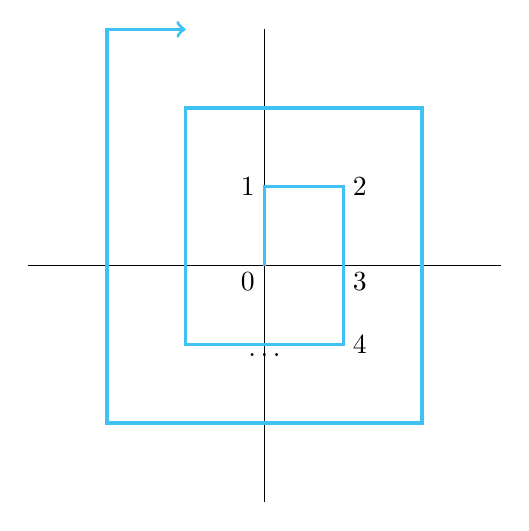
\begin{tikzpicture}
\draw (-3, 0) -- (3, 0);
\draw (0, -3) -- (0, 3);
\draw[cyan!75, very thick, ->] (0, 0) -- (0,1) -- (1,1) -- (1,0) -- (1, -1) -- (0, -1) -- (-1, -1) -- (-1, 0) -- (-1, 1) -- (-1, 2) -- (0, 2) -- (1, 2) -- (2,2) -- (2,1) -- (2, 0) -- (2, -1) -- (2, -2) -- (1, -2) -- (0, -2) -- (-1, -2) -- (-2, -2) -- (-2, -1) -- (-2, 0) -- (-2, 1) -- (-2, 2) -- (-2, 3) -- (-1, 3); 
\draw (0,-0.2) node[anchor=east]{$0$};
\draw (0, 1) node[anchor=east]{$1$};
\draw (1, 1) node[anchor=west]{$2$};
\draw (1, -0.2) node[anchor=west]{$3$};
\draw (1, -1) node[anchor=west]{$4$};
\draw (0, -1) node[anchor=north]{$\ldots$};
\end{tikzpicture}
\end{center}
By construction, this determines a bijection.
\end{proof}
\begin{exercise}
Determine an explicit piecewise formula for the bijection $f: \N \to \Z$ in the proof above.
\end{exercise}

In general, we note that $\Z^n$ is countable by considering spirals in higher dimensions. However, the reader may already expect this to be true --- there is enough space between lattice points in order to have $|\Z^n| = \aleph_0$. However, $\Q$ is dense, in that in between any two rational numbers, there exists a third rational number. Hence, it is reasonable to expect $\Q$ to have a larger cardinality, but we will show something certainly upsetting, at least to mathematicians in the early 20th century.
\begin{theorem}
$\Q$ is countable.
\end{theorem}
\begin{proof}[Proof of a Special Case]
We just discuss the rational interval $I := [0, 1] \cap \Q$. We enumerate this set by first considering the and denominator:
$$I = \set{\frac 01, \frac 11, \frac 02, \frac 12, \frac 22, \frac 03, \frac 13, \frac 23, \frac 33, \frac 04, \frac 14, \frac 24, \frac 34, \cdots}.$$
We simply delete the duplicates off the list to get an enumeration of $I$:
$$I = \set{0, 1, \frac 12, \frac 13, \frac 14, \frac 14, \frac 34, \frac 15, \frac 25, \frac 35, \cdots}.$$
\end{proof}
Using a careful enough ``spiral," we can show that $\Q$ is countable. However, we will state the following principle, which shows that deleting the duplicates was not actually necessary.

\begin{proposition}
Let $X$ be a set. If there exists a surjection $f: \N\to X$, then $X$ is countable.
\end{proposition}
\begin{exercise}
In the case that $X$ is infinite, provide a proof of the statement above by finding a bijection $g: \N\to X$ using the surjection $f: \N\to X$ given.
\end{exercise}

One may ask, are there sets too large to be countable? The answer is \textit{yes} --- there are in fact sets larger than $\Q$ that cannot be put into bijection with the natural numbers.
\begin{definition}
A set $A$ is \textit{uncountable} if it is not countable.
\end{definition}
Of course, this set must be infinite in size. We are already familiar with one such uncountable set: the real numbers.
\begin{theorem}
$\R$ is uncountable.
\end{theorem}
\begin{proof}
Obviously $(0, 1)\subseteq \R$. We first show that $(0, 1)$ is uncountable. Assume for contradiction that $(0, 1)$ is countable. Hence write
$$(0, 1) = \set{x_1, x_2, x_3, x_4,\ldots},$$
which is an enumeration of the set $(0, 1)$. Write each $x_i$ in its infinite decimal expansion\footnote{That is, if $x_i = 1/4$, then write $x_i = 0.24\overline 9$ instead of $x_i=0.25$.} and arrange them as such. By assumption, this list consists of all elements of $(0, 1)$:
\begin{align*}
x_1 &= 0.a_{11}a_{12}a_{13}a_{14}a_{15}\ldots \\
x_2 &= 0.a_{21}a_{22}a_{23}a_{24}a_{25}\ldots \\
x_3 &= 0.a_{31}a_{32}a_{33}a_{34}a_{35}\ldots \\
x_4 &= 0.a_{41}a_{42}a_{43}a_{44}a_{45}\ldots \\
\vdots
\end{align*}
For our contradiction, we produce an element $x$ that does not lie on the list. Define the digit $b_i$ to be given by $b_i = 4$ if $a_{ii}\neq 4$ and $b_i = 5$ if $a_{ii} = 4$, and set $x = 0.b_1b_2b_3b_4b_5\ldots$. We see that $x$ disagrees with each $x_i$ at the $i$th decimal place; hence, it cannot be on the list. Yet $b_i \in (0, 1)$, a contradiction. Hence, $(0, 1)$ is be uncountable. Now, consider the chain of functions
$$(0, 1) \overset f\longrightarrow \paren{-\frac \pi2, \frac\pi2} \overset g\longrightarrow \R$$
where $f(x) := -\frac \pi2 + \pi x$ and $g(x) := \tan x$. The reader can show that both $f$ and $g$ are bijections, so that $g\circ f$ is also a bijection. Hence $\abs{(0, 1)} = |\mathbb R|$, so $\R$ is uncountable.
\end{proof}

\newpage
The argument we used to prove that $(0, 1)$ was uncountable is known as a \textit{diagonal argument}, due to how we only considered the digits $a_{ii}$, which appear on the diagonal of our hypothetical list we made above.

\begin{exercise}
Using a similar diagonal argument, prove that $\mathcal P(\N)$ is uncountable. However, show that the set of all \textit{finite} subsets of $\N$ is in fact \textit{countable}.
\end{exercise}

Recall that our definition of cardinality requires that we find a bijection between two sets. However, in the uncountable case, this is often difficult, but we have the following theorem. We will not prove the theorem, and we recommend the reader read the various proofs online.
\begin{theorem}[Cantor-Schr\"oder-Bernstein Theorem]
Let $A,B$ be sets. If there exist injections $f: A\to B$ and $g: B\to A$, then there exists a bijection $h: A\to B$.
\end{theorem}
In short, the theorem states that if $|A| \leq |B|$ and $|B| \leq |A|$, then $|A| = |B|$. This statement is surely true for numbers and for finite cardinalities, though it is not a triviality for infinite sets. We view some examples.

\begin{example}
We show that $(0, 1)$ and $(0,1)^2$ have the same cardinality. For one, notice that $f: (0, 1)\to (0,1)^2$ by $x\mapsto (x, 1/2)$ is an injection by construction. Now, we find an injection $g: (0,1)^2\to (0,1)$. Notice that every element $x\in (0,1)$ has a unique decimal expansion, as long as we always choose the non-terminating expansion when necessary. Now, define $g: (0,1)^2 \to (0,1)$ such that if $x = 0.d_1d_2d_3\ldots$ and $y = 0.e_1e_2e_3\ldots$, we have
$$g(x,y) = 0.d_1e_1d_2e_2d_3e_3\ldots.$$
Again, $g$ is injective by construction. Hence $\abs{(0,1)} = \abs{(0,1)^2}$.
\end{example}

\begin{exercise}
Prove that the set of all \textit{infinite binary sequences} (i.e., sequences of $0$'s and $1$'s) is uncountable without a diagonalization argument.
\end{exercise}

Now, we turn to a third way of determining countability: by using a set's subsets. We have already done this to some extent when we showed that $\R$ contained an uncountable subset, but we did so by constructing an explicit bijection between that subset and $\R$. The next few theorems show us that we can skip this step, but we first introduce some notation.
\begin{definition}
Let $I$ be a set, and to each $i\in I$ assign a set $A_i$. That is, the sets $A_i$ are \textit{indexed} by the set $I$. We define the \textit{indexed union} by
$$\bigcup_{i\in I} A_i := \Big\{x: (\exists i\in I)\, x\in A_i\Big\}$$
and the \textit{indexed intersection} by
$$\bigcap_{i\in I} A_i := \Big\{x: (\forall i\in I)\, x\in A_i\Big\}.$$
\end{definition}
We note that in the case that $I = \Z^+$, we often write $\ds\bigcup_{i=1}^\infty A_i$ (and similarly for intersections) in place of the notation presented here. However, when we are proving something about a union or intersection indexed by $\Z^+$, \textbf{you \underline{may not} write}
$$\bigcup_{i=1}^\infty A_i = A_1 \cup A_2 \cup A_3 \cup \cdots$$
\textbf{and attempt to manipulate the expression on the right-hand side}, no matter how true it seems --- that is \textbf{not} the definition of the indexed union, though it is a useful shorthand, even if the notation is technically abusive. We demonstrate this principle in the proof of the theorem below.

\begin{theorem}
A union of countably many countable sets is countable. That is, if $A_1, A_2, A_3,\ldots$ is a sequence of countable sets, then $\ds\bigcup_{i=1}^\infty A_i$ is countable.
\end{theorem}
\begin{proof}
Let $A := \ds\bigcup_{i=1}^\infty A_i$. We construct a surjection $f: \N\to A$, so by Proposition 16.6, we are done. We note that $A_i\subseteq A$ for every $i\in\Z^+$,\footnote{Prove this statement carefully.} so it follows that we can just list the elements of $A$, grouped by the $A_i$:
\begin{align*}
 A_1 &= \set{a_{11}, a_{12}, a_{13}, \ldots} \\
 A_2 &= \set{a_{21}, a_{22}, a_{23}, \ldots} \\
 A_3 &= \set{a_{31}, a_{32}, a_{33}, \ldots}
\end{align*}
Now, count the elements by going diagonally across from right to left: send $1\mapsto a_{11}, 2\mapsto a_{12}, 3\mapsto a_{21}, 4\mapsto a_{13}, 5\mapsto a_{22}, 6\mapsto a_{31}$, and so on and so forth. This gives a surjection $f: \N\to A$, so we are done.
\end{proof}

\begin{example}
Let $S$ be the set of natural-number sequences with finitely many nonzero terms. We show that $S$ is countable.
\end{example}
\begin{proof}
Define $S_n := \ds\set{(x_0, x_1, x_2,\ldots)\in S: \sum_{i=0}^\infty x_i = n}$. Of course, because only finitely many terms in each sequence is nonzero, the sum converges, so our definition is valid. Then, we see that
$$S = \bigcup_{n\in\N} S_n,$$
as no sum of the sequences in $S$ can possibly diverge. We claim that each of the $S_n$'s are countable. To each $n\in\N$, fix some $m\in\N$ with $m \leq n$, and consider the set $S_n(m)$ given by
$$S_n(m) := \set{x\in S_n: x \textrm{ has exactly } m \textrm{ nonzero terms}}.$$
We leave it for the reader to verify that each $S_n(m)$ is indeed countable, and that
$$S_n = \bigcup_{m=1}^n S_n(m),\footnote{This is an honest finite union $S_n(1)\cup S_n(2)\cup \cdots \cup S_n(n)$.}$$
hence $S_n$ is countable. By the preceding theorem, we are done.
\end{proof}

Our next theorem allows us to quickly establish uncountability.
\begin{theorem}
If $A$ is uncountable and $B$ is countable, then $A\setminus B$ is uncountable.
\end{theorem}
\begin{proof}
Notice that $A = (A\setminus B)\cup (A\cap B)$. Clearly, $A\cap B$ is countable. Now, assume for contradiction that $A\setminus B$ is countable. Then the restriction Theorem 16.12 to finite unions would imply $A$ is countable, a contradiction. Hence $A\setminus B$ is uncountable.
\end{proof}
\newpage
\begin{example}
The irrational numbers $\R\setminus \Q$ are uncountable, as $\Q$ is countable while $\R$ is not.
\end{example}

In fact, we can say something slightly stronger than the previous theorem.
\begin{theorem}
If $A$ is infinite and $B$ is countable, and $A\setminus B$ is infinite, then $\abs{A\setminus B} = \abs A$.
\end{theorem}
\begin{proof}
Since $A$ is infinite, $A$ must contain a countably infinite subset.\footnote{That is, $\aleph_0$ is the ``smallest" infinity. See the exercises at the end of this section.} Since $B$ is countable, so is $A\cap B$, so we enumerate
$$A\cap B = \set{b_0, b_1, b_2, b_3, \ldots}.$$
Now, define $S := \set{a_0, a_1, a_2, \ldots} \subseteq A\setminus B$. We consider two cases.

\textit{Case I:} If $A\cap B$ is finite, there is basically no work to be done.

\textit{Case II:} If $A\cap B$ is infinite, define the function $f: A\to A\setminus B$ by
$$f(x) = \begin{cases}
    x & x\not\in (A\cap B) \cup S \\
    a_{2n+1} & x = b_n \text{ for some } n\in\N \\
    a_{2n} & x = a_n \text{ for some } n \in \N.\\
\end{cases}$$
We leave it for the reader to show that $f$ is indeed injective. Now, the embedding $g: A\setminus B\to A$ by $g(x) = x$ is obviously injective, so by Cantor-Schr\"oder-Bernstein, we are done.
\end{proof}

Similarly, the following holds as well.
\begin{proposition}
If $A$ is infinite and $B$ is countable, then $|A\cup B| = |A|$.
\end{proposition}
\begin{exercise}
Prove the above proposition, using a similar argument as to Theorem 16.16.
\end{exercise}
\subsection*{Infinite Infinities}
Thus far, we have only seen two types of infinities: countable infinity $\aleph_0$ and the size of the real numbers $\R$, sometimes known as the \textit{continuum} (denoted $\mathfrak c$). However, we can continue building larger and larger infinities, using the power set operation. Recall that the power set gives as a notion of exponentiation (with base $2$), which gives us larger sets. This is even true for \textit{infinite} sets, as we shall see in the theorem and proof below.
\begin{theorem}[Cantor's Theorem]
Let $X$ be any set. then $|X| < |\mathcal P(X)|$.
\end{theorem}
\begin{proof}
We have already proved the finite case, so suppose $X$ is infinite. First, we know $|X| \leq |\mathcal P(X)|$, as we have the embedding $f: X \to \mathcal P(X)$ by $x\mapsto \set{x}$. Now, assume for contradiction that $|\mathcal P(X)| = |X|$; i.e., there is a bijection between elements of $X$ and subsets of $X$. If $g$ is such a bijection, we denote $g(x) = A_x$. Define
$$R := \set{x\in X: x\not\in A_x}\subseteq X,$$
that is, $R$ contains all elements of $X$ that are not contained in their image $A_x$. Since $R\subseteq X$, we have $R = A_y$ for some $y\in X$. Now, the question is, does $R$ contain $y$?

If $y\in R$, then $y\not\in A_y$ by definition of $R$. But $A_y = R$, a contradiction. Similarly, if $y\not\in R$, then $y\not\in A_y$, but by definition of $R$, $y\in R$, a contradiction. Hence, the existence of the bijection causes a contradiction, so we must have $|X| < |\mathcal P(X)|$.
\end{proof}
\newpage
This allows us to build a chain of increasing infinities.
\begin{corollary}
There exists an infinite sequence of infinite sets $A_1, A_2, A_3, \ldots$ such that $$|A_1| < |A_2| < |A_3| < \cdots.$$
\end{corollary}
\begin{proof}
Take $A_1 = \N$, $A_2 = \mathcal P(\N)$, and inductively take $A_n = \mathcal P(A_{n-1})$ for $n\geq 2$. By Cantor's Theorem, we have $|A_n| < |A_{n+1}|$ for all $n\geq 1$, so we are done.
\end{proof}

\subsection*{Conclusion: Transcendental Numbers}
We finish these notes with a discussion of polynomials and their relation to cardinality. Let us start with the following definitions.
\begin{definition}
A complex number $\alpha$ is \textit{algebraic} if it is a root of a polynomial with integer coefficients. 
\end{definition}
For the sake of notation, we denote the set of all polynomials with integer coefficients by $\Z[x]$. Hence, $\alpha$ is algebraic if there exists some $f\in \Z[x]$ such that $f(\alpha) = 0$.

\begin{definition}
Let $\alpha\in\C$ be algebraic. The \textit{degree} of $\alpha$ is the minimal degree of a polynomial $f\in \Z[x]$ such that $\alpha$ is a root of $f$.
\end{definition}

\begin{example}
Suppose $\alpha$ has (algebraic) degree $1$. Hence $\alpha$ is the root of some $ax + b\in\Z[x]$, $a\neq 0$, i.e., $\alpha = -b/a\in\Q$. In fact, this shows that $\alpha\in \Q$ is equivalent to $\alpha$ being algebraic of degree $1$. Similarly, if $\beta$ is algebraic of degree $2$, then it is the root of some $ax^2+bx+c\in \Z[x]$, $a\neq 0$, so that by the quadratic formula
$$\beta = \frac{-b\pm \sqrt{b^2-4ac}}{2a},$$
taking either plus or minus as necessary.
\end{example}

\begin{definition}
We say $\alpha\in\C$ is \textit{transcendental} if it is not algebraic.
\end{definition}
In abstract algebra, ``not algebraic" is sometimes formulated as ``if $f(x)\in \Z[x]$ satisfies $f(\alpha) = 0$, then $f = 0$." [The reader may show that this is equivalent.] Transcendental numbers are notoriously hard to find, and it is always a hefty task to show that a number is not algebraic, as there are infinitely many polynomials $\Z[x]$ of arbitrarily high degree. To give a little bit of history:
\begin{itemize}
    \item Johann Heinrich Lambert \textit{conjectured} in 1761 that $\pi$ was transcendental.
    \item Joseph Liouville showed that transcendental numbers actually existed in 1844, and he found the example $L := \ds\sum_{n=1}^\infty \frac 1{10^{n!}}$.
    \item Charles Hermite showed that $e$, the base of the natural logarithm, was transcendental in 1873.
    \item Ferdinand von Lindemann, over a century after it was conjectured, finally proved that $\pi$ was transcendental in 1882. He first showed that $e^\alpha$ was transcendental when $\alpha$ was algebraic.\footnote{This statement is today known as the Lindemann-Weierstrass Theorem, with Karl Weierstrass proving a more general case.} Since $e^{\pi i} = -1$, it follows that $\pi i$ is transcendental, hence $\pi$ is transcendental.
\end{itemize}

Additionally, to this day (2024) we only know that at least one of $e+\pi$ and $e\pi$ is transcendental, yet we find ourselves unable to conclusively say which one(s) is/are transcendental. For certain other types of numbers, we have even worse luck than this.
\begin{definition}
Let $s\in\C$. We define the \textit{Riemann zeta function} to be the sum
$$\zeta(s) := \sum_{n=1}^\infty \frac 1{n^s} = \frac 1{1^s} + \frac 1{2^s} + \frac 1{3^s} + \frac 1{4^s} + \cdots,$$
where the domain of $\zeta$ is any place in the complex plane where the infinite sum converges.
\end{definition}
Euler proved in 1735 that $\zeta(2) = \pi^2/6$ in the famous Basel problem, yet it was by Lindemann's result that $\zeta(2)$ was shown to be transcendental. In 1978, Roger Apéry showed that $\zeta(3)$, now known as \textit{Apéry's constant} in his honor, is \textit{irrational} --- it is still open whether it is algebraic or transcendental. Similarly, we are unsure whether the very important numbers
$$G := \sum_{i=0}^n \frac{(-1)^n}{(2n+1)^2} =  \frac 1{1^2} - \frac 1{3^2} + \frac 1{5^2} - \frac 1{7^2}+ \cdots \text{ (Catalan's Constant) and}$$
$$\gamma := \lim_{n\to\infty}\paren{-\ln n + \sum_{k=1}^n \frac 1k} \text{ (Euler-Mascheroni Constant)}$$
are even irrational, let alone transcendental. Hence, we may jump to the conclusion that transcendental numbers are very rare among the complex numbers, and that most numbers are at the very least algebraic. However, our final theorem in these notes show that this is in fact not the case --- most complex numbers \textit{are} transcendental! This is somewhat of a scary thought: most of the numbers we even think about form a tiny subset of $\R$, let alone $\C$ --- the ``average" number is virtually indescribable with our vocabulary.

\begin{theorem}
There are uncountably many transcendental numbers, while there are only countably many algebraic numbers.
\end{theorem}
\begin{proof}
Let $\mathbb A$ denote the set of algebraic numbers, and let $\mathbb A_d$ denote the set of algebraic numbers with degree $d$. Then
$$\mathbb A = \bigcup_{d=1}^\infty \mathbb A_d.$$
It thus suffices to show that each $\mathbb A_d$ is countable. Fixing $d\in \Z^+$, every polynomial in $\Z[x]$ with degree $d$ has at most $d$ unique roots, so it is enough to show that there are only countably infinitely many polynomials with degree $d$. Now, each polynomial $c_dx^d+c_{d-1}x^{d-1} + c_1x + c_0\in\Z[x]$ is uniquely determined by the sequence of coefficients $(c_d, c_{d-1}, \ldots, c_1, c_0)\in \Z^{d+1}$; i.e., we have found a bijection between the set of all polynomials in $\Z[x]$ with degree \textit{at most $d$} and $\Z^{d+1}$. We know that $\Z^{d+1}$ is countably infinite, so that the set of all polynomials with degree at most $d$ is countably infinite, and thus the number of polynomials wth degree exactly $d$ is countable, hence $\mathbb A_d$ is countable. This implies $\mathbb A$ is countable, so that $\C\setminus\mathbb A$, the set of transcendental numbers, is uncountable as $\C$ is uncountable.
\end{proof}

We end with David Hilbert's quote on Cantor's results which we explored in this section: ``From the paradise, that Cantor created for us, no one shall be able to expel us."

\newpage
\subsection*{Exercises}
\begin{exercise}
Show that a set is infinite if and only if there exists a subset of size $n$ for every $n\geq 1$.
\end{exercise}

\begin{exercise}
Let $A$ be a set. Show that the following statements are equivalent:
\begin{enumerate}
    \item $A$ is infinite.
    \item $A$ has a countably infinite subset.
    \item $A$ has a \textit{proper} subset $B$ satisfying $|B| = |A|$.
\end{enumerate}
This exercise shows that \textit{all} infinite sets have the unintuitive property that they contain a strictly ``smaller" set with the same size, and this property is \textit{necessary and sufficient} for a set to be infinite. [We have used this many times in the proofs of the theorems in the main text.]
\end{exercise}

\begin{exercise}
We define $\Q(\sqrt 2, \sqrt 3) := \set{\sqrt 2r + \sqrt 3s: r,s\in \Q}$. Show that there exist infinitely many $c\in\R$ such that $3^x\ln y + 5^y\cos x = c$ has no solution $x,y\in\Q(\sqrt 2,\sqrt 3)$.
\end{exercise}

\begin{exercise}
Let $f: (0, 1]\to (0,1)$ be given by
$$f(x) := \begin{cases}
1/(n+1) & t=1/n \textrm{ for some } n\in\N \\
t & \textrm{otherwise.}
\end{cases}$$
Show that $f$ is a bijection. [This gives an explicit bijection between $(0, 1]$ and $(0, 1)$.]
\end{exercise}

\begin{exercise}
Construct an explicit bijection $f: (0,1) \to [0, 1]$.
\end{exercise}
\begin{exercise}
Are each of these following sets finite, countably infinite, or uncountably infinite?
\begin{itemize}
    \item[(a)] $\Q(x) = \{p(x)/q(x): p, q\in \Q[x]\}$, where $\Q[x]$ is the set of polynomials with rational coefficients.
    \item[(b)] $\R[x]$, the set of polynomials with real coefficients.
    \item[(c)] The set of finite subsets of $\R$.
    \item[(d)] The set of continuous functions on $\R$.
\end{itemize}
\end{exercise}

\begin{exercise}
Let $S\subseteq\R^2$ be the set of all points $(x,y)$ such that $x^2+y^2 = a^2$ and $y=bx$ for some $a,b\in\Q$. Is $S$ countable?
\end{exercise}
\begin{exercise}
Are the following sets finite, countably infinite, or uncountably infinite?
\begin{itemize}
    \item[(a)] The set of all lines in $\R^2$ having rational slope and rational $y$-intercept.
    \item[(b)] The set of circles in $\R^2$ having rational radii and centers with rational coordinates.
\end{itemize}
\end{exercise}
\begin{exercise}
Let $f: \R\to\Q$. Show that there exists an uncountable subset $S\subseteq\R$ such that $f(x) = f(y)$ for every $x,y\in S$.
\end{exercise}
\newpage

\begin{exercise}
This exercise provides an alternate proof that the algebraic numbers are countable. Again, use $\mathbb A$ to denote the algebraic numbers.
\begin{itemize}
    \item[(a)] Let $M\in\Z^+$. Show that there are finitely many choices of $d\in\Z^+$ and $a_0,\ldots, a_d\in \Z$ with $M = d + \ds\sum_{k=0}^d |a_k|$.
    \item[(b)] Let $P_M := \{a_dx^d + \cdots + a_1x + a_0: M = d + |a_0| + |a_1| + \cdots + |a_d|\}$. Why is $P_M$ \textit{finite}?
    \item[(c)] We know that every polynomial of degree $d$ has at most $d$ distinct roots in $\C$. Show that $R_M := \{x\in\R: p(x) = 0 \textrm{ for some }p\in P_M\}$ is finite.
    \item[(d)] Prove that $\mathbb A = \ds\bigcup_{M=1}^\infty R_M$, which completes the proof.
\end{itemize}
\end{exercise}

\begin{exercise}
In this exercise we show that if $|A| < \aleph_0$, then $A$ is finite. Suppose for contradiction that $A$ is an infinite set satisfying $|A| < \aleph_0$, so there exists an injection $f: A\to\Z^+$. Enumerate the elements in the range of $f$ in increasing order: $\im f = \{n_1, n_2,n_3,\ldots\},$ where $n_i<n_j$ if $i<j$.
\begin{itemize}
    \item[(a)] Prove that $\im f$ is infinite.
    \item[(b)] Show that for all $k\in\Z^+$, there exists a unique $a_k\in A$ with $f(a_k) = n_k$.
    \item[(c)] Define $g: \Z^+\to A$ by $g(k) = a_k$. Prove that $g$ is a bijection, and hence deduce a contradiction.
\end{itemize}
\end{exercise}

\begin{exercise}
Let $X$ be a nonempty set and $\A\subseteq \mathcal P(X)$. We say that $\A$ is a $\sigma$-\textit{algebra} if it satisfies the following 3 conditions:
\begin{enumerate}
    \item $\varnothing, X\in\A$.
    \item If $S\in \A$, then $S^c\in \A$. (We treat $X$ as the universal set.)
    \item If $S_1, S_2,\ldots\in \A$, then their union is in $\A$.
\end{enumerate}
This exercise shows that countably infinite $\sigma$-algebras cannot exist. We proceed by contradiction: suppose $\A = \{S_1, S_2,S_3,\ldots\}$ is countably infinite, and assume the sets $S_i$ are all distinct.
\begin{itemize}
    \item[(a)] Show that the universal set $X$ is infinite.
    \item[(b)] For each $x\in X$, define $B_x := \ds \bigcap_{\{n\in\N: x\in S_n\}} S_n$. Show that $B_x\in\A$ for any $x\in X$.
    \item[(c)] Show that if $E\in\A$ and $x\in E$, then $B_x\subseteq E$. That is, show that $B_x$ is the smallest set in $\A$ containing $x$.
    \item[(d)] Let $x,y\in X$. Suppose $B_x\cap B_y \neq \varnothing$ and let $z\in B_x\cap B_y$. Show $x,y\in B_z$, so that $B_x = B_y = B_z$. That is, show that two sets $B_x, B_y$ are either disjoint or equal.
    \item[(e)] Show that there exists a sequence $x_1, x_2, x_3, \ldots$ in $X$ such that $x_i\neq x_j$ if $i\neq j$.
    \item[(f)] Deduce a contradiction by constructing an injection from the set of binary sequences into $\A$.
\end{itemize}
\end{exercise}
\begin{exercise}
Give an example of an uncountable set $I$ and $\{A_t: t\in I\}$ such that each each $A_t$ is countably infinite and the following $3$ conditions hold: (1) if $s\neq t$, then $A_s\neq A_t$, (2) for all $s,t$, either $A_s\subseteq A_t$ or $A_s\supseteq A_t$, and (3) $\bigcup_{t\in I} A_t$ is countably infinite.
\end{exercise}

\section*{References}
Though these notes are largely independent of the official Math 13 notes, some of the material here can be found there as well: \url{https://www.math.uci.edu/~ndonalds/math13/notes.pdf}.
\end{document}
